\documentclass[Protokollheft.tex]{subfiles}
\begin{document}
\chapter{Elektrostatik und Magnetostatik 1}
%--------------- Start Vorbereitungsaufgaben ---------------
\section{Vorbereitungsaufgaben}

{\subsection{Elektrostatik}}

% --> Aufgabe
\begin{framed}
	\noindent \textbf{1.} An welchen Stellen im Gitter sind jeweils die elektrischen
Spannungen $\efit$, die Potentiale $\varphi$, die Ladungen $q$ und die
dielektrischen Flüsse $\dfit$ in der Elektrostatik allokiert?\label{exer:allocateElectrical}
\end{framed}
\noindent
Die elektrischen Spannungen $\efit$ sind auf den primären Kanten definiert. Die elektrische Flussdichte $\dfit$ ist dagegen auf den dualen Flächen allokiert. Passend zu den elektrischen Spannungen, sind die Potentiale $\varphi$ auf den primären Knoten definiert. Die Ladungen $q$ sind in den dualen Volumen allokiert.

% --> Aufgabe
\begin{framed}
	\noindent \textbf{2.} Machen Sie sich anhand einer lokalen \emph{zweidimensionalen}
Betrachtung die Beziehung zwischen der Ladung $q_n$ einer dualen Zelle $n$ und
den assoziierten Potentialen klar. Skizzieren
Sie dazu zunächst das lokale Gauß'sche Gesetz für eine duale
Zelle. Nutzen Sie dabei anstatt der auftretenden Feldkomponenten 
die diskreten Potentialwerte, die Sie durch Gradientenbildung aus den 
Feldkomponenten erhalten (siehe Gleichung (4.11)).\\
Betrachten Sie dazu zunächst ein äquidistantes Gitter mit
Schrittweite $\Delta s$ und eine homogene Materialverteilung mit der
Permittivität $\eps_0$. Tragen Sie den entstehenden
"`Differenzenstern"' (Differenzen der beteiligten Potentialwerte,
die mit den Kopplungskoeffizienten gewichtet werden) in Ihre
Skizze ein.\label{exer:diffStar}
\end{framed}
\noindent
Betrachtet man zunächst die diskrete Potentialgleichung
\begin{equation*}
\divdfit\Meps\divdfit^\top\varphi=\mathbf{q},
\end{equation*}
so kann man diese auch umschreiben zu
\begin{equation*}
	\Meps\divdfit\divdfit^\top\varphi=\mathbf{q},
\end{equation*}
da $\Meps$ eine Diagonalmatrix ist. Da es homogene Materialverteilung und ein äquidistantes Gitter angenommen wird vereinfacht sich die Gleichung zu
\begin{equation*}
	\divdfit\divdfit^\top\varphi=\frac{1}{\Delta s\varepsilon_0}\mathbf{q}.
	\label{eq:SSphi}
\end{equation*}
Daraus lässt sich nun einfach der Differenzenstern ableiten. Dieser entsteht durch das Produkt $\divdfit\divdfit^\top$. Ausgehend vom Gauß'schen Gesetz für die duale Fläche
\begin{equation*}
\int_{\partial \tilde{A}}\vec{D}\cdot\text{d}\vec{s}=\mathbf{q}
\end{equation*}
erhält man durch einsetzen der diskreten elektrischen Flussdichten $\dfit$
\begin{equation*}
-\dfit_{n-1}+\dfit_{n}-\dfit_{n+n_p-1}+\dfit_{n+n_p}=\mathbf{q}_n.
\end{equation*}
durch Umschreiben in elektrische Feldstärken $\efit$ erhält man
\begin{equation*}
	-\efit_{n-1}+\efit_{n}-\efit_{n+n_p-1}+\efit_{n+n_p}=\frac{1}{\Delta s\varepsilon_0}\mathbf{q}_n.
\end{equation*}
Die elektrischen Feldstärken kann man nun wieder mit Hilfe des Gradienten in Potentiale umwandeln.
\begin{eqnarray*}
	-(-(\varphi_n-\varphi_{n-1})+(\varphi_{n+1}-\varphi_n)-(\varphi_n-\varphi_{n-n_x})+(\varphi_{n+n_x}-\varphi_n))&=&\frac{1}{\Delta s\varepsilon_0}\mathbf{q}_n\\
	4\varphi_n-\varphi_{n-1}-\varphi_{n+1}-\varphi_{n+n_x}-\varphi_{n-n_x}&=&\frac{1}{\Delta s\varepsilon_0}\mathbf{q}_n\\
\end{eqnarray*}
Diese Formulierung entspricht genau einer Zeile der Gleichung \ref{eq:SSphi}. Der dazu passende geometrische Differenzenstern ist in Abbildung \ref{fig:diffstern} zu sehen.


% --> Aufgabe
\begin{framed}
	\noindent \textbf{3.} Betrachten Sie nun den Fall nichtäquidistanter Gitter
und inhomogener Materialverteilung, also die Werte der Materialmatrix im
Differenzenstern. Veranschaulichen Sie sich die Struktur der Systemmatrix $\mathbf{A}$ mit Hilfe einer Skizze der Bandstruktur.\label{exer:bandsOfSystemMat}
\end{framed}
\noindent
Im Fall nichtäquidistanter Gitter ändern sich die Gewichtungen der einzelnen Werte im Differenzenstern. Die Struktur bleibt aber immer erhalten. Schuld für die Änderungen der Gewichte ist die Materialmatrix $\Meps$. Allein durch sie ändern sich die Gewichte. Ist das Material homogen und isotrop, so kann der Wert für $\varepsilon$ einfach auf die andere Seite der Gleichung gebracht werden (vgl. Gleichung \ref{eq:SSphi}). Ist dies nicht der Fall, so muss die Materialmatrix an den Differenzenstern multipliziert werden. Die Materialverteilung kann nun in jeder Zelle anders sein. Die Materialbeziehung zwischen $\dfit$ und $\efit$ ändert sich nun zu
\begin{equation*}
	\dfit_n=\frac{\bar{\varepsilon}|\tilde{A}_n|}{|L_n|}\efit_{n}.
\end{equation*}
Die Permittivität korreliert also mit dem Flächeninhalt der dualen Fläche $\tilde{A}_n$ und mit der Länge der primären Kante $L_n$. Genau dieser Faktor ist entscheidend für die Gewichtung innerhalb des Differenzensterns.

% --> Aufgabe
\begin{framed}
	\noindent \textbf{4.} Gegeben sei ein zweidimensionales Rechengebiet mit den
Abmessungen\footnote{Alle Größen hier und im Folgenden in SI-Einheiten.} $0.6\times 1.2$ mit        
dem Koordinatenursprung bei $(0,0)$. Es seien drei Punktladungen im
Rechengebiet mit $q_1=q_0$ am Punkt $(0.3,0.2)$,  $q_2=q_0/2$ bei
$(0.6,0.4)$, und  $q_3=q_0/4$ bei $(0.9,0.2)$ gegeben.\\
Berechnen Sie die Größe und den Ort des Ladungsschwerpunkts $q_{\text{S}}$. Das
Rechengebiet sei homogen mit $\eps_0$ gefüllt und äquidistant mit
$3 \times 4$ Gitterzellen diskretisiert. Berechnen Sie außerdem die
Potentiale der Randknoten so, dass die Problemstellung mit einer
offenen Berandung versehen ist.\label{exer:averagePointCharges}
\end{framed}

Die Große des Ladungsschwerpunkts bestimmt man mit Sumation alle Ladungen in betretenem Gebiet.
$$ q_{\text{S}}=q_1 + q_2 + q_3= \frac{7}{4}q_0 $$
Der Ort des Ladungsschwerpunkts bestimmt man mit dem Formel:
$$\vec{r_\text{S}}=\begin{bmatrix}
x_{\text{S}} \\
 y_{\text{S}}  
\end{bmatrix}=
\frac{\begin{bmatrix}
	x_{\text{1}} \\
	y_{\text{1}}  
	\end{bmatrix}q_1+
\begin{bmatrix}
x_{\text{2}} \\
y_{\text{2}}  
\end{bmatrix}q_2+
\begin{bmatrix}
x_{\text{3}} \\
y_{\text{3}}  
\end{bmatrix}q_3}{q_{\text{S}}}=
\frac{\begin{bmatrix}
	0.3 \\
	0.2  
	\end{bmatrix}q_0+
	\begin{bmatrix}
	0.6 \\
	0.4  
	\end{bmatrix}\frac{q_0}{2}+
	\begin{bmatrix}
	0.9 \\
	0.2  
	\end{bmatrix}\frac{q_0}{4}}{\frac{7}{4}q_0}=
\begin{bmatrix}
0.471 \\
0.257  
\end{bmatrix}
$$
Das Gabiet hat insgesamt 14 Randknoten und Potenzial an der Rand des homogenen Gebietes rechnet man mit der Formel:

$$\varphi_\text{Rand}(\vec{r_\text{S}},\vec{r})=\frac{q_\text{S}}{4\pi\varepsilon_0\vert\vert \vec{r}-\vec{r_\text{S}}\vert\vert} $$  
Mit der Formel erhält man:
\begin{eqnarray}
\vec{r_1}=\begin{bmatrix}
0 \\
0    
\end{bmatrix} \text{ :       }\varphi_\text{Rand}(\vec{r_\text{S}},\vec{r_1})= 2.9314 \cdot 10^{10}q_0\\
\vec{r_2}=\begin{bmatrix}
0.3 \\
0    
\end{bmatrix} \text{ :       }\varphi_\text{Rand}(\vec{r_\text{S}},\vec{r_2})= 5.0952 \cdot 10^{10}q_0\\
\vec{r_3}=\begin{bmatrix}
0.6 \\
0    
\end{bmatrix} \text{ :       }\varphi_\text{Rand}(\vec{r_\text{S}},\vec{r_3})= 5.4697 \cdot 10^{10}q_0\\
\vec{r_4}=\begin{bmatrix}
0.9 \\
0    
\end{bmatrix} \text{ :       }\varphi_\text{Rand}(\vec{r_\text{S}},\vec{r_4})= 3.1451 \cdot 10^{10}q_0\\
\vec{r_5}=\begin{bmatrix}
1.2 \\
0    
\end{bmatrix} \text{ :       }\varphi_\text{Rand}(\vec{r_\text{S}},\vec{r_5})= 2.0348 \cdot 10^{10}q_0\\
\vec{r_6}=\begin{bmatrix}
0 \\
0.2    
\end{bmatrix} \text{ :       }\varphi_\text{Rand}(\vec{r_\text{S}},\vec{r_6})= 3.3152 \cdot 10^{10}q_0\\
\vec{r_{10}}=\begin{bmatrix}
1.2 \\
0.2    
\end{bmatrix} \text{ :       }\varphi_\text{Rand}(\vec{r_\text{S}},\vec{r_{10}})= 2.151 \cdot 10^{10}q_0\\
\vec{r_{11}}=\begin{bmatrix}
0 \\
0.4    
\end{bmatrix} \text{ :       }\varphi_\text{Rand}(\vec{r_\text{S}},\vec{r_{11}})= 3.1954 \cdot 10^{10}q_0\\
\vec{r_{15}}=\begin{bmatrix}
1.2 \\
0.4    
\end{bmatrix} \text{ :       }\varphi_\text{Rand}(\vec{r_\text{S}},\vec{r_{15}})= 2.1172 \cdot 10^{10}q_0\\
\vec{r_{16}}=\begin{bmatrix}
0 \\
0.6    
\end{bmatrix} \text{ :       }\varphi_\text{Rand}(\vec{r_\text{S}},\vec{r_{16}})= 2.6994 \cdot 10^{10}q_0\\
\vec{r_{17}}=\begin{bmatrix}
0.3 \\
0.6    
\end{bmatrix} \text{ :       }\varphi_\text{Rand}(\vec{r_\text{S}},\vec{r_{17}})= 4.1035 \cdot 10^{10}q_0\\
\vec{r_{18}}=\begin{bmatrix}
0,6 \\
0.6    
\end{bmatrix} \text{ :       }\varphi_\text{Rand}(\vec{r_\text{S}},\vec{r_{18}})= 4.2921 \cdot 10^{10}q_0\\
\vec{r_{19}}=\begin{bmatrix}
0.9 \\
0.6    
\end{bmatrix} \text{ :       }\varphi_\text{Rand}(\vec{r_\text{S}},\vec{r_{19}})= 2.863 \cdot 10^{10}q_0\\
\vec{r_{20}}=\begin{bmatrix}
1.2 \\
0.6    
\end{bmatrix} \text{ :       }\varphi_\text{Rand}(\vec{r_\text{S}},\vec{r_{20}})= 1.9523 \cdot 10^{10}q_0
\end{eqnarray} 

% --> Aufgabe
\begin{framed}
	\noindent \textbf{5.} Berechnen Sie, wenn möglich, die Kapazitäten folgender Anordnungen mithilfe von Kondensatorschaltungen. Die Abmessung soll für alle Anordnungen mit $1\times1\times1$     
angenommen werden. Dabei befinden sich die Elektroden bei $y = 0$ und $y = 1$. Wie kann Anordnung e) geändert werden, damit sie mit einer Kondensatorschaltung berechnet werden kann?
\begin{enumerate}[label=\alph*)]
\item Homogen mit Permittivität $\eps_\text{r}=1$.
\item Äquidistant längsgeschichtet mit Permittivitäten $\eps_{\text{r}1}=1$ und $\eps_{\text{r}2}=2$                    (Reihenschaltung).
\item Äquidistant quergeschichtet mit Permittivitäten $\eps_{\text{r}1}=1$ und $\eps_{\text{r}2}=2$                     (Parallelschaltung).
\item Längs- und quergeschichtet mit Permittivitäten $\eps_{\text{r}1}=1$,                      
$\eps_{\text{r}2}=2$, $\eps_{\text{r}3}=3$ und $\eps_{\text{r}4}=4$ (Reihenschaltung von Parallelschaltungen bzw. Parallelschaltung von Reihenschaltungen).
\item Homogen gefüllter Kondensator ($\eps_\text{r}=1$) mit Zick-Zack-förmiger oberer Platte. Ausgehend von einem homogenen Plattenkondensator soll die Geometrie der oberen Platte durch das Einbringen eines metallischen Quaders mit den Punkten $(0,0.5,0)$ und $(0.5,1,1)$ modelliert werden.
\end{enumerate}
\label{exer:calcCapsAnalytical}
\end{framed}
Um Kapazität einer Platenkondesator zu ausrechnen, benutzt man dieser Formel:
$$\text{C}=\varepsilon_r\varepsilon_0\frac{A}{l} $$
$\text{A}$ bezeichnet Fläche einer Platte un $\text{l}$ die Abstand zwischen zweier Platten.

\begin{enumerate}[label=(\alph*)]
	\item Hier hat man  einfaches Plattenkondensator mit  $\text{A}=1$ und $\text{l}=1$.\\
	$$\text{C}=\varepsilon_0=8.54\mathrm{pF}$$
	\item Hier hat man ein Reihenschaltung zweier Kondensatoren mit $\text{A}=1$ und $\text{l}=0.5$ 
	$$\text{C}=2\varepsilon_0\frac{\varepsilon_1\varepsilon_2}{\varepsilon_1+\varepsilon_2}=\frac{2}{3}\varepsilon_0= 5.8\mathrm{pF}$$
	\item Hier hat man ein Parallelschaltung zweier Kondensatoren mit $\text{A}=0.25$ und $\text{l}=1$ 
	 $$\text{C}=\frac{1}{4}\varepsilon_0(\varepsilon_1+\varepsilon_2)=\frac{3}{4}\varepsilon_0=6.64\mathrm{pF}$$
	\item  Hier hat man ein Parallelschaltung von Reihenschaltungen vier Kondensatoren mit $\text{A}=0.25$ und $\text{l}=0.5$
	$$\text{C}=\frac{1}{2}\varepsilon_0\left[\frac{\varepsilon_1\varepsilon_2}{\varepsilon_1+\varepsilon_2}+\frac{\varepsilon_3\varepsilon_4}{\varepsilon_3+\varepsilon_4} \right]=\frac{25}{21}\varepsilon_0=10.54\mathrm{pF}$$
\end{enumerate}

\newpage
%
{\subsection{Skalare Magnetostatik}}

% --> Aufgabe
\begin{framed}
	\noindent \textbf{6.} An welcher Stelle im Gitter müssen die Komponenten des Gitterstroms
$\jfit$ allokiert werden (bei gegebenem Ansatz des magnetischen Skalarpotentials)?\label{exer:allocateCurrent}
\end{framed}
\noindent
Da die diskrete magnetische Feldstärke $\hfit$ auf den primären Kanten definiert ist, ist die diskrete Stromdichte $\jfit$ als über die Divergenzmatrix $\mathbf{S}$ mit $\mathbf{S}\hfit = \jfit$, verbundene Größe auf den primären Flächen definiert. 


% --> Aufgabe
\begin{framed}
	\noindent \textbf{7.} Berechnen Sie analytisch das magnetische Feld um einen unendlich
ausgedehnten Linienleiter und skizzieren Sie die zu erwartende
Feldverteilung.\label{exer:HfieldAroundLineConductor}
\end{framed}
\noindent
Aus dem amperischen Gesetz für die Magnetostatik
\begin{equation}
	\label{eq:ampere}
	\int_{\partial A} \vec{H} \cdot \text{d}\vec{s} = \int_A \vec{J} \cdot \text{d} \vec{A} 
\end{equation}
ergibt sich durch Transformation der linken Seite in Zylinderkoordinaten und auflösen der rechten Seite
\begin{equation*}
	\int_{0}^{2\pi} \varrho\ \vec{H} \cdot \vec{e_\varphi}   \ \text{d} \varphi = I.
\end{equation*}
Durch auflösen des Integrales, umstellen nach $H_\varphi$ und einsetzen in das Materialgesetz $\vec{H} = \mu \vec{B}$  ergibt sich somit
\begin{equation}
	\label{eq:bLeiter}
	B_\varphi = \frac{I}{2\mu \pi \varrho} %  an????
\end{equation}


% --> Aufgabe
\begin{framed}
	\noindent \textbf{8.} Wie können die Dirichlet- und die Neumann- Randbedingung physikalisch gedeutet werden, wenn sie in der Magnetostatik auf das magnetische Skalarpotential angewandt werden?\label{exer:bndCondMagScalarPot}
\end{framed}
\noindent
Bei einer physikalischen Deutung der Dirichlet-Randbedingungen für ein magnetisches Feld lassen sich diese als Übergang zu einem Material perfekter magnetischer Leitfähigkeit interpretieren, welches alle Feldlinien in sich hineinzieht, weshalb die Felder senkrecht in den Rand übergehen. \\
Neuman-Randbedingungen lassen sich hingegen als perfekter elektrischer Leiter an den Ränder interpretieren, der alle Feldlinien aus sich herausdrängt, weshalb die Felder senkrecht in den Rand übergehen.  

% --> Aufgabe
\begin{framed}
	\noindent \textbf{9.} Das Problem eines unendlich langen Leiters ist ein
offenes 2D-Problem und müsste durch eine offene
Randbedingung in der FIT modelliert werden. Wenn das
Rechengebiet hinreichend groß ist, kann ohne großen
Genauigkeitsverlust für die Felder im Inneren des Rechengebiets
auf die komplizierte Implementierung eines offenen Randes
verzichtet werden. Welche Randbedingung eignet sich hierfür besser? (Neumann ($H_{\text{n}}=0$) oder Dirichlet ($\vec{H}_{\text{t}}=0$))?\label{exer:boundCondInfiniteConductor}
\end{framed}
\noindent
Für die Approximation eines Linienleiters im freien Raum durch setzen von Rändern in hinreichend großer Entfernung eignen sich Neumann- besser als Dirichlet-Randbedingungen.\\
Dies ist darin begründet das es sich beim approximierten Feld, wie in Abb. \ref{fig:neumannrand} zu sehen, um ein Zylindrisches Feld handelt. Da die bei Neumannrandbedingungen die normale Komponente $\vec{H}_n$ des Feldes am Rand verschwindet und nur die Tangentialkomponente auftritt, verlaufen Feldvektoren des simulierten Feldes schon in weiten Teilen in eine ähnliche Richtung wie an den Grenzflächen und werden durch diese nur im geringen Maße, vor allem an den Ecken, gestört. \\
Wie in \ref{fig:dirichletrand} zu sehen, führen Dirichletrandbedinungen hier zu einer deutlichen Verzerrung des Feldes in der Nähe des Randes.   


%TODO

\section{Aufgaben während der Praktikumssitzung}

{\subsection{Elektrostatik}}

Kern dieses Abschnitts bildet die Implementierung eines Solvers für elektrostatische
Probleme. Anhand der Kondensatoranordnungen aus der Vorbereitung können die
Routinen mit analytischen Berechnungen verglichen und das Konvergenzverhalten
untersucht werden. Der Kondensator mit Knick dient darüber hinaus als Beispiel
für ein analytisch nicht lösbares Problem.

% --> Aufgabe
\begin{framed}
	\noindent \textbf{1.} Vervollständigen Sie die in \lstinline{solveES.m} vorgegebene Funktion
\begin{align}
\lstinline{[phi, ebow, dbow, relRes] = solveES(msh, eps, pots, q, bc)} \; ,
\end{align}
welche einem allgemeinen Elektrostatik-Solver entspricht. \lstinline{msh} ist hierbei das Rechengitter, \lstinline{eps} die Permittivität, \lstinline{pots} die gesetzten Potentiale für jeden Gitterpunkt (nicht bekannte Potentiale sind mit dem Wert \lstinline{NaN} in diesem Vektor gekennzeichnet), \lstinline{q} die vorgegebenen Ladungen und \lstinline{bc} die vorgegebenen Randbedingungen. \lstinline{phi}, \lstinline{ebow} und \lstinline{dbow} sind die integralen Feldgrößen und \lstinline{relRes} ist ein Vektor mit den relativen Residuen des Solvers in jedem Iterationsschritt.\\
\ \\
{\textbf{Hinweis:}} Für die Implementierung werden Ihnen einige Routinen vorgegeben
(zum Teil handelt es sich um optimierte Funktionen aus vergangenen Versuchen), welche auf den nächsten Seiten beschrieben sind. Verwenden Sie diese so oft wie möglich.\label{exer:solveES}
\end{framed}


% --> Aufgabe
\begin{framed}
	\noindent \textbf{2.} Schreiben Sie eine Methode
\begin{align}
\lstinline{cap = calcCap(msh, ebow, dbow)} \; ,
\end{align}
die die Kapazität \lstinline{cap} berechnet und zurück gibt. Verwenden Sie hierzu die vorgegebenen Methoden \lstinline{intEdge} und
\lstinline{intSurf}.\label{exer:calcCap}
\end{framed}


% --> Aufgabe
\begin{framed}
	\noindent \textbf{3.} Verwenden Sie nun die letzten beiden Methoden in dem teilweise vorgegebenen Skript \lstinline{exampleCaps.m}, um
die Kapazität der Kondensatorkonfigurationen a) bis d) der Vorbereitungsaufgaben numerisch zu berechnen und mit Ihren analytischen Ergebnissen zu vergleichen. Hängt die Lösung von der Größe des Gitters ab?\label{exer:calcCapNumerically}
\end{framed}
\noindent
Mit Hilfe der vorherigen Implementationen können wir nun die Kapazitäten der 5 Kondensatoren aus Aufgabe \ref{exer:calcCapsAnalytical}.1 5 numerisch bestimmen.
\begin{eqnarray*}
C_a &=& -4.058083\ \text{pF}\\
C_b &=& -4.058083\ \text{pF}\\
C_c &=& -8.116167\ \text{pF}\\
C_d &=& -6.885970\ \text{pF}\\
C_e &=& -1.014140\ \text{pF}\\
\end{eqnarray*}
\noindent
Durch eine Verfeinerung des Gitters verändern sich die Werte unwesentlich.

% --> Aufgabe
\begin{framed}
	\noindent \textbf{4.} Visualisieren Sie im selben Skript das Potential (\lstinline{plotPotential}) und das elektrische Feld (\lstinline{plotEdgeVoltage})
der fünf Kondensatorkonfigurationen. Wählen Sie hierfür eine sinnvolle Diskretisierung und eine zweidimensionale Darstellung mit sinnvoller Schnittebene~\lstinline{indz}. Kommentieren Sie kurz die Feldbilder im Hinblick auf die analytischen Feldverläufe.\label{exer:visualizeCapField}
\end{framed}
\noindent
Die Feldverläufe und Potentiale der Kondensatoren sind in den Abbildungen \ref{fig:potA} bis \ref{fig:C_5e_3D} zu sehen. Sie entsprechen weitestgehend den analytischen Feldbildern und Potentialen.

% --> Aufgabe
\begin{framed}
	\noindent \textbf{5.}   Dokumentieren Sie das Konvergenzverhalten des iterativen Solvers für Kondensatorkonfiguration~e), indem Sie
den Verlauf des relativen Residuums als Funktion des Iteratonsschritts $n_\text{iter}$ mithilfe eines Matlab-Skripts \lstinline{plotConv.m} grafisch darstellen.\\
{\textbf{Hinweis:}} Entsprechend Vorgabe ist das relative Residuum für jeden Iterationsschritt in \lstinline{relRes} enthalten.\label{exer:plotCapConvSolver}
\end{framed}
\noindent
Wie in Abb. \ref{fig:residiumiIterationen} zu erkennen nimmt das relative Residuum exponentiell mit der Anzahl der Iterationen ab. 
Beim relativen Residuum handelt es sich um die Differenz zwischen der $i$-ten und $(i-1)$-ten Iteration. 





% --> Aufgabe
\begin{framed}
	\noindent \textbf{6.} Schreiben Sie nun ein Skript \lstinline{plotConvCap.m}, das die letzte Kondensatorkonfiguration e) numerisch berechnet
und zusätzlich das Konvergenzverhalten (hier nicht vom Gleichungssystemlöser, sondern von der Gitterverfeinerung)
angibt. Stellen Sie auch diese Lösung wieder grafisch dar.\\
Welcher Unterschied besteht zwischen der Konvergenz des iterativen Solvers und der Verbesserung der Lösungsgenauigkeit durch zunehmende Gitterzellenanzahl, der sogenannten Verfahrenskonvergenz?\label{exer:plotCapConvMesh}
\end{framed}
\noindent
Durch eine Verfeinerung des Gitters kann, wie in Abb. \ref{fig:kapazitaetueberanzstuetzstellen} zu erkennen, eine Annäherung in Form einer Kehrwertfunktion $\frac{1}{np}$ erreicht werden. \\
Verglichen mit der exponentiellen Annäherung durch die Anzahl der Iterationsschritte, ist dies zwar deutlich langsamer, da aber die Iterationsschritte sich immer nur an die, durch die Anzahl der Stützstellen begrenzte, Genauigkeit annähern können, ist in der praktischen Anwendung eine Kombination aus beidem notwendig. 

%
{\subsection{Skalare Magnetostatik}}
Analog zur Elektrostatik wird nun ein Solver für magnetostatische Probleme implementiert, welcher das magnetische Skalarpotential verwendet. Das Rechengebiet wird erneut zu $1\times 1\times 1$ gewählt. In der Mitte des Rechengebietes soll sich ein in $z$-Richtung das komplette Rechengebiet durchlaufender Linienleiter, der den Strom \SI{1000}{A} führt, befinden.

% --> Aufgabe
\begin{framed}
	\noindent \textbf{7.} Verwenden Sie die vorgegebene Methode \lstinline{calcHi}, um das Hilfsfeld $\hfit_{\text{i}}$ des Linienleiters zu berechnen.
Stellen Sie es grafisch dar. Nutzen Sie für diese Implementierung bitte das gegebene Skript \lstinline{exampleHi.m}.\label{exer:visualizeHi}
\end{framed}

Graphische Darstellung befindet sich in Abbildung \ref{fig:hilffeld}.

% --> Aufgabe
\begin{framed}
	\noindent \textbf{8.} Vervollständigen Sie den Solver
\begin{align}
\lstinline{[hbow, bbow, relRes] = solveMS(msh, mu, jbow, bc)} \; ,
\end{align}
wobei \lstinline{mu} hier die Permeabilität, \lstinline{jbow} der Gitterstromfluss und
\lstinline{hbow} bzw. \lstinline{bbow} die Feldgrößen sind.\\
\ \\
{\textbf{Hinweis:}} Verwenden Sie wieder die vorgegebenen Routinen sowie die \matlab-Datei \lstinline{solveMS}. Benutzen Sie
dafür u.\,A. die Routine \lstinline{createMeps} und beachten Sie die vertauschte Allokation der Felder in der skalaren Magnetostatik.\label{exer:solveMS}
\end{framed}



% --> Aufgabe
\begin{framed}
	\noindent \textbf{9.} Verwenden Sie \lstinline{solveMS} um das $\vec{H}$-Feld zu berechnen und grafisch darzustellen. Nutzen Sie für diese Implementierung bitte das Skript \lstinline{exampleMShomogen.m}. Entspricht das Feldbild Ihren Erwartungen?\label{exer:visualizeHfield}
\end{framed}

Feldbild in Abb. \ref{fig:homfeld} sieht aus wie erwartet. Es soll ein radialsymmetrisches Wirbelfeld sein.

% --> Aufgabe
\begin{framed}
	\noindent \textbf{10.} Wählen Sie ein einfaches (aber sinnvolles) Beispiel einer inhomogenen Materialverteilung. Verwenden Sie die vorhandenen Methoden, um das
Problem zu lösen und grafisch darzustellen. Nutzen Sie für diese Implementierung bitte das Skript \lstinline{exampleMSinhomogen.m}.\label{exer:Hfield4inhomogenMaterial}
\end{framed}

Graphische Darstellung inhomogenes $\vec{H}$-Feldes ist in Abbildung \ref{fig:inhomfeld}.



\section{Fazit}
In diesem Versuch haben wir mit Magnetostatik und Elektrostatik beschäftigt. Wir haben die $\vec{E}$- und $\vec{H}$-Felder mittels FIT- Methode ausgerechnet. 

\clearpage
\newpage
\section{Abbildungen}
\begin{figure}[h!]
	\centering
	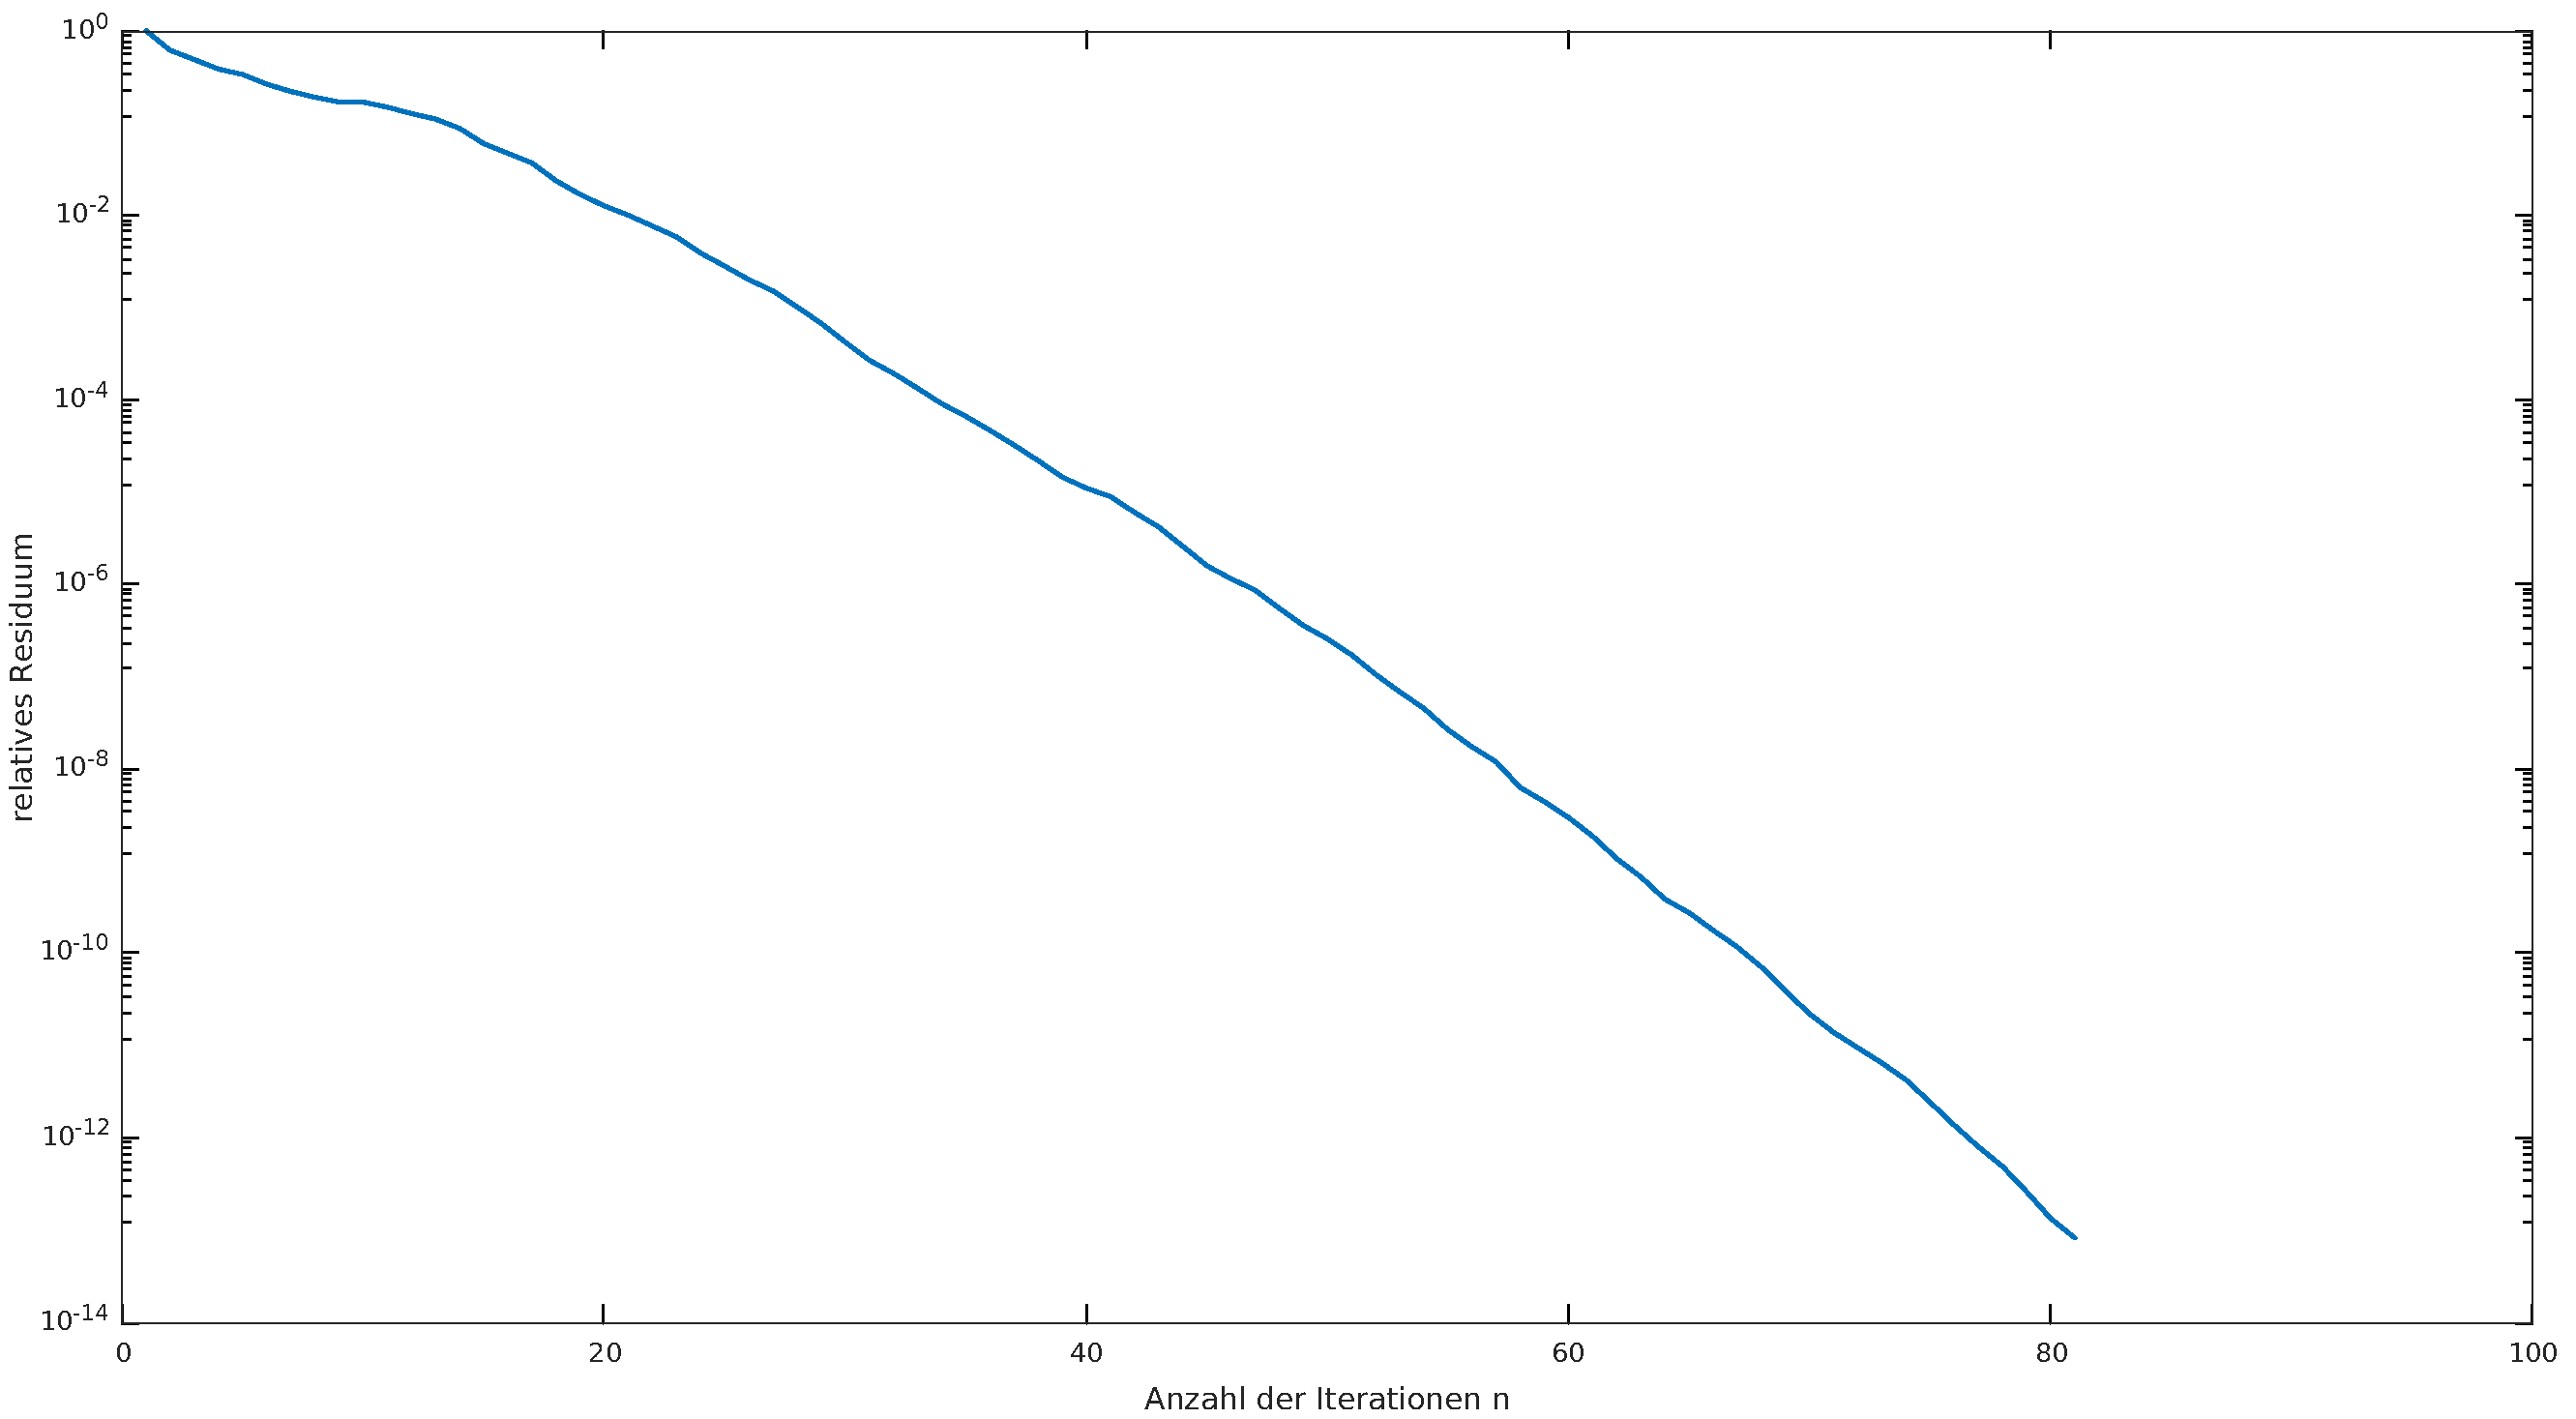
\includegraphics[width=0.7\linewidth]{ResidiumIterationenGraph.pdf}
	\caption{Verlauf des relativen Residuums für einen iterativen Solvers über der Anzahl der Iterationsschritte am Beispiel der Berechnung eines Kondensators}
	\label{fig:residiumiIterationen}
\end{figure}

\begin{figure}[h!]
	\centering
	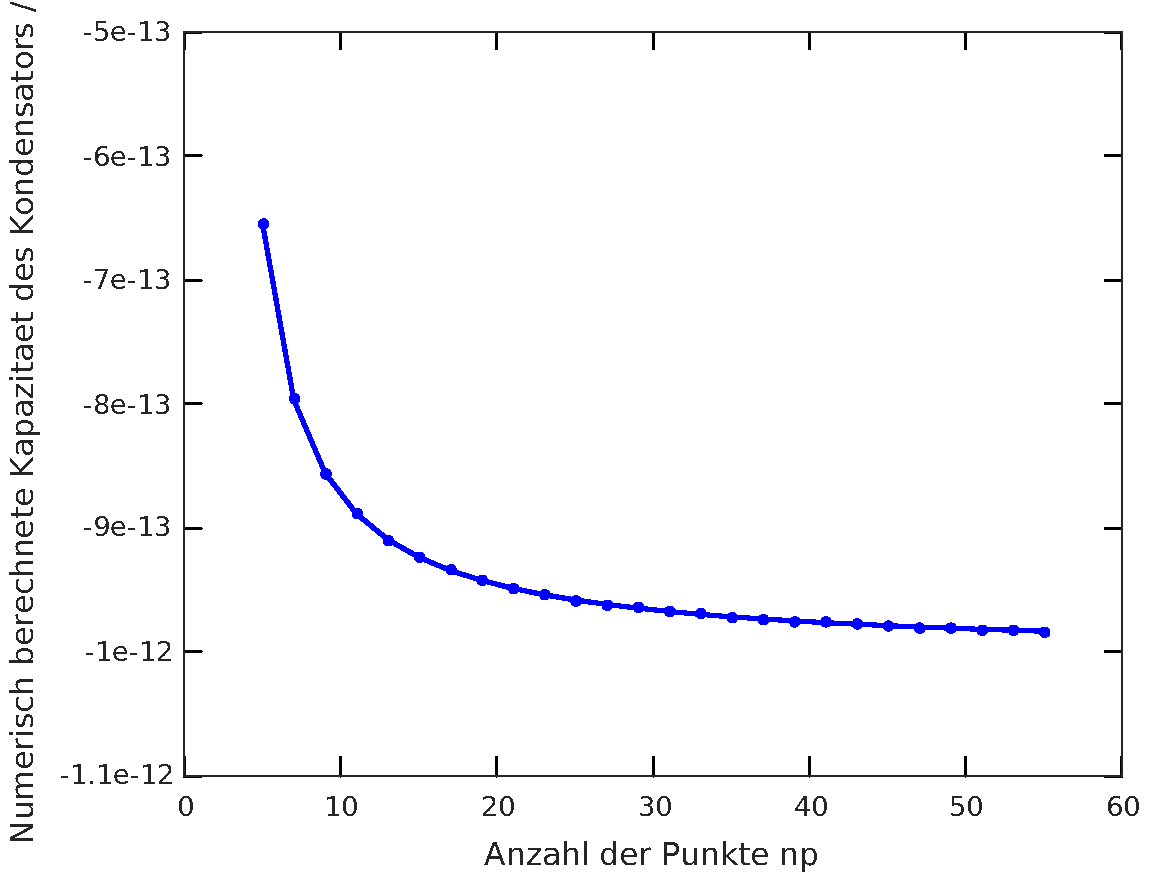
\includegraphics[width=0.7\linewidth]{KapazitaetUeberAnzStuetzstellen.pdf}
	\caption{Nummerisch bestimmte Kapazität eines Kondensators in Abhängigkeit von der Anzahl der Stützstellen}
	\label{fig:kapazitaetueberanzstuetzstellen}
\end{figure}

\begin{figure}[h!]
	\centering
	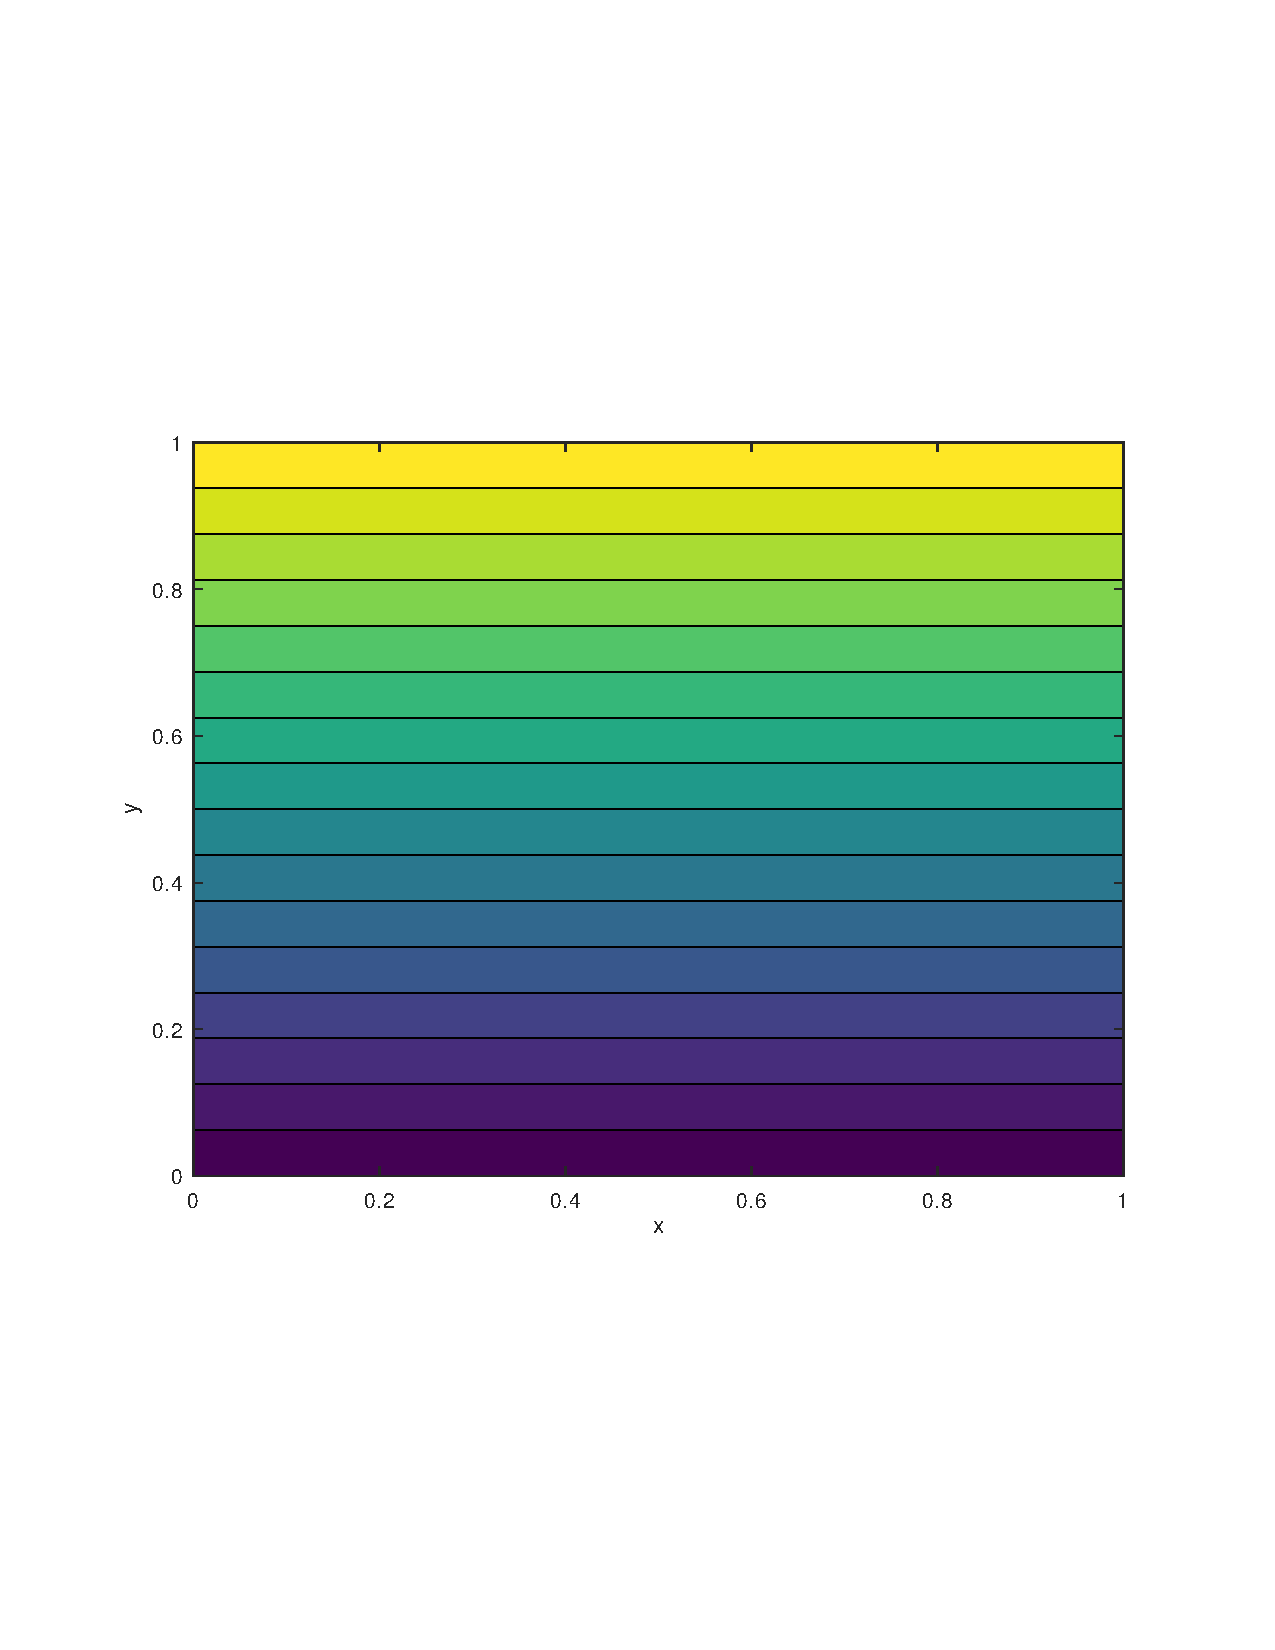
\includegraphics[trim = 20mm 70mm 20mm 70mm, clip,width=0.7\linewidth]{potential_A.pdf}
	\caption{Numerisch bestimmter Potentialverlauf des Kondensators aus \ref{exer:calcCapsAnalytical}.1 5a$)$}
	\label{fig:potA}
\end{figure}

\begin{figure}[h!]
	\centering
	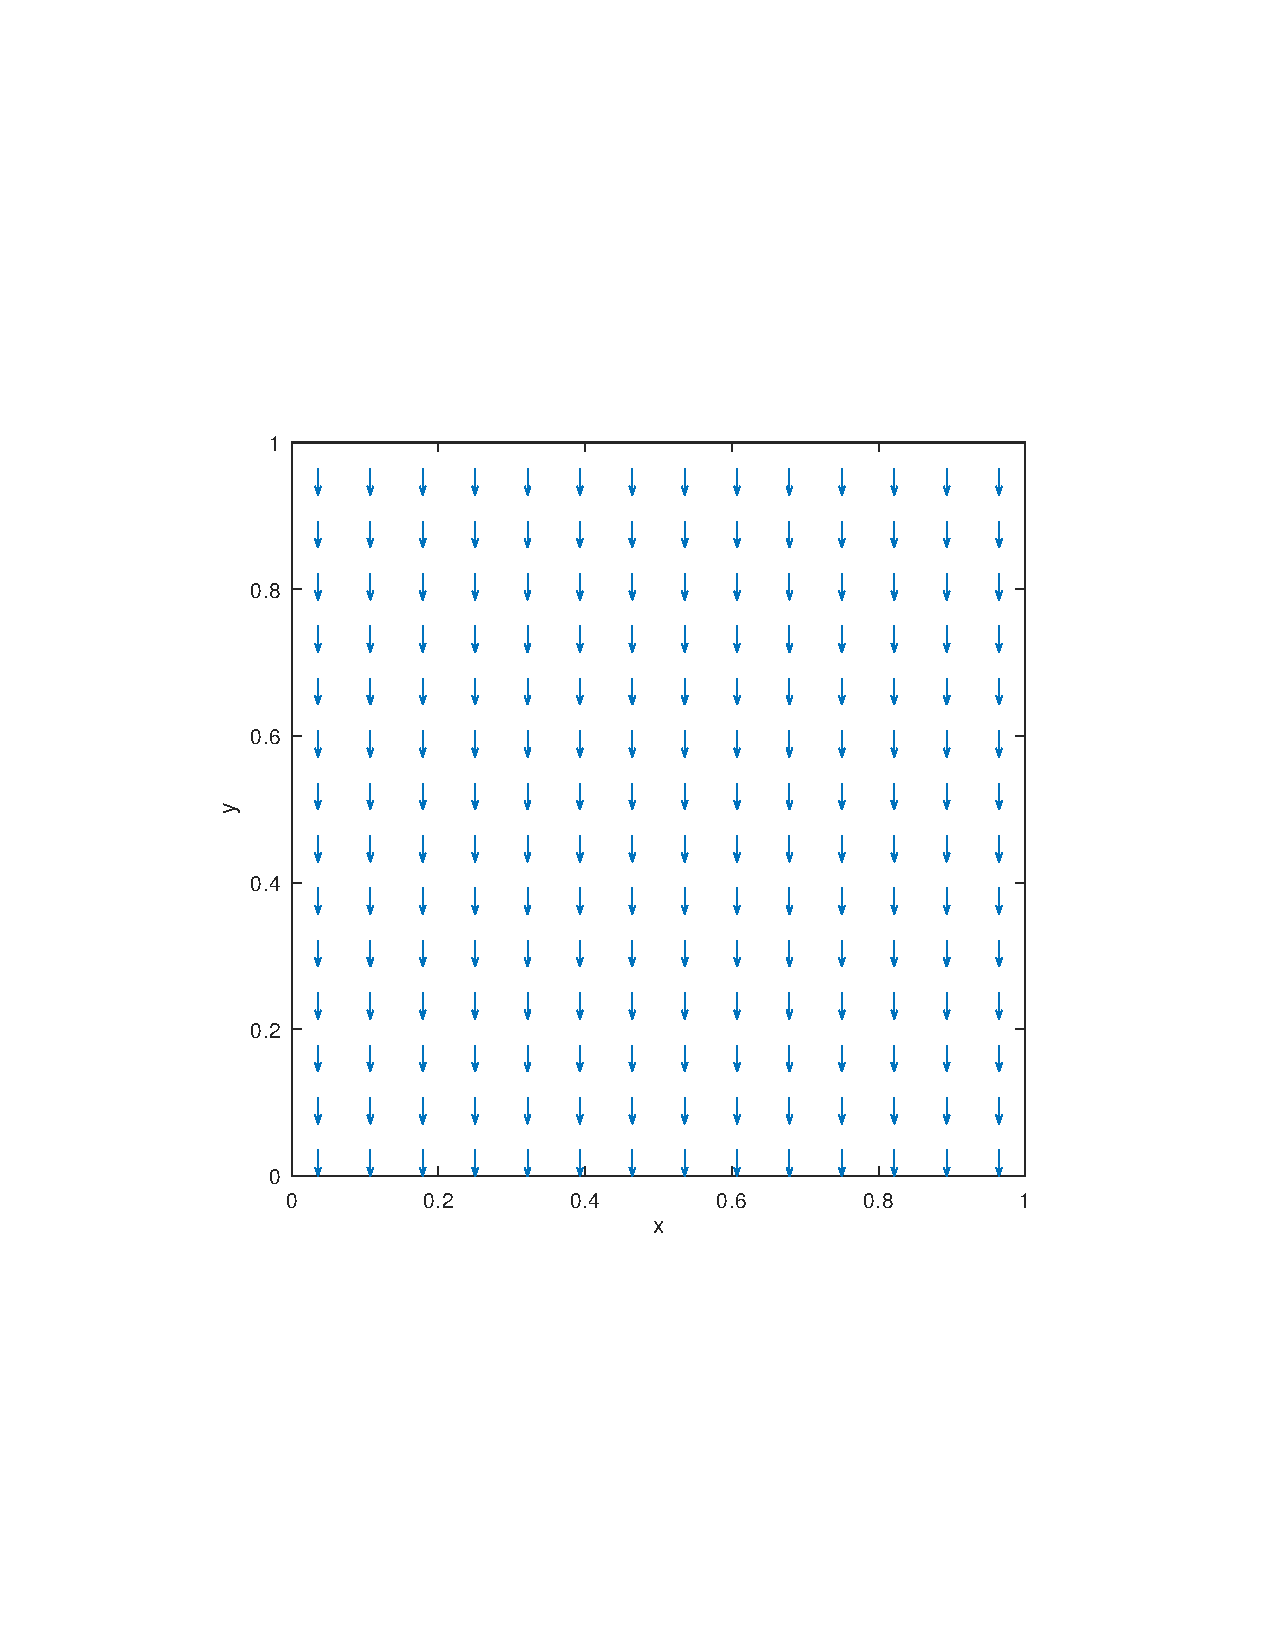
\includegraphics[trim = 20mm 70mm 20mm 70mm, clip,width=0.7\linewidth]{E_2D_A.pdf}
	\caption{Numerisch bestimmter Verlauf des elektrischen Feldes des Kondensators aus \ref{exer:calcCapsAnalytical}.1 5a$)$ in 2D}
	\label{fig:potA}
\end{figure}

\begin{figure}[h!]
	\centering
	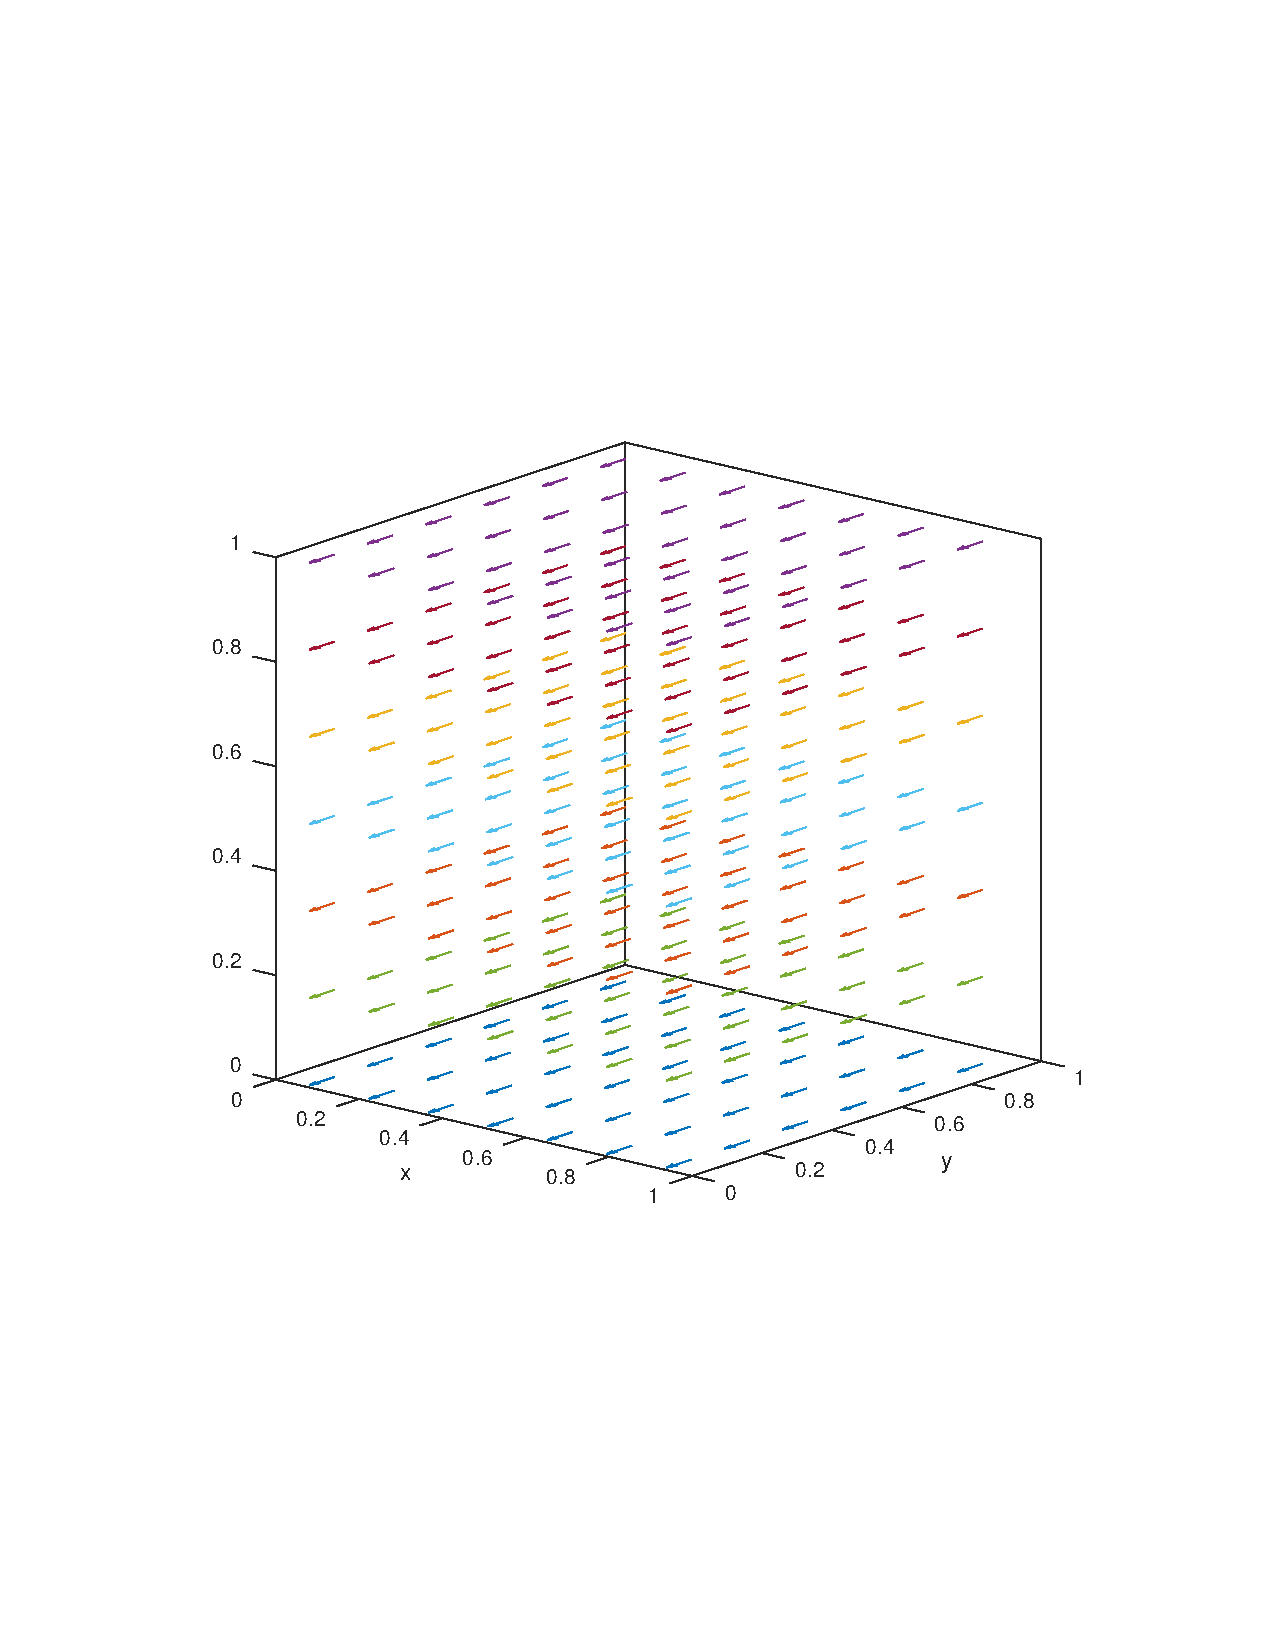
\includegraphics[trim = 20mm 70mm 20mm 70mm, clip,width=0.7\linewidth]{E_3D_A.pdf}
	\caption{Numerisch bestimmter Verlauf des elektrischen Feldes des Kondensators aus \ref{exer:calcCapsAnalytical}.1 5a$)$ in 3D}
	\label{fig:potA}
\end{figure}

\begin{figure}[h!]
	\centering
	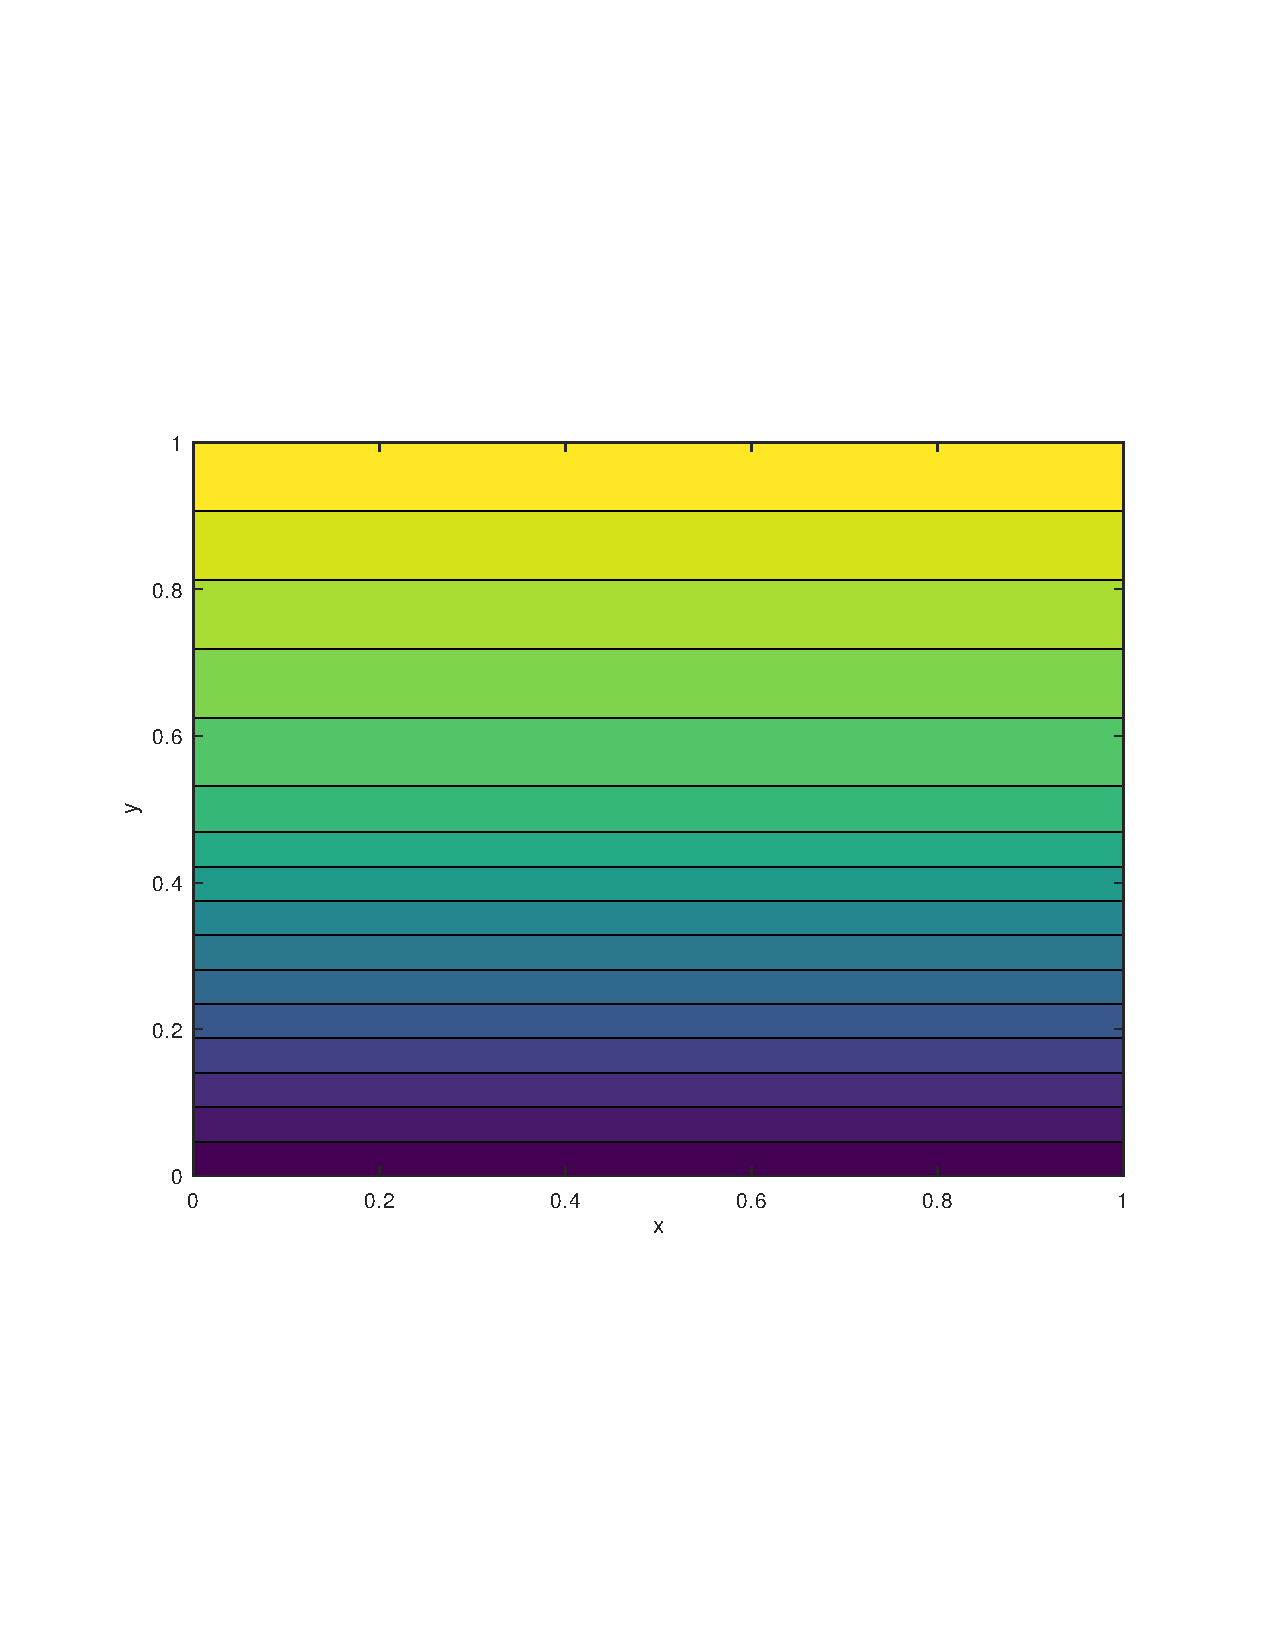
\includegraphics[trim = 20mm 70mm 20mm 70mm, clip,width=0.7\linewidth]{potential_B.pdf}
	\caption{Numerisch bestimmter Potentialverlauf des Kondensators aus \ref{exer:calcCapsAnalytical}.1 5b$)$}
\end{figure}

\begin{figure}[h!]
	\centering
	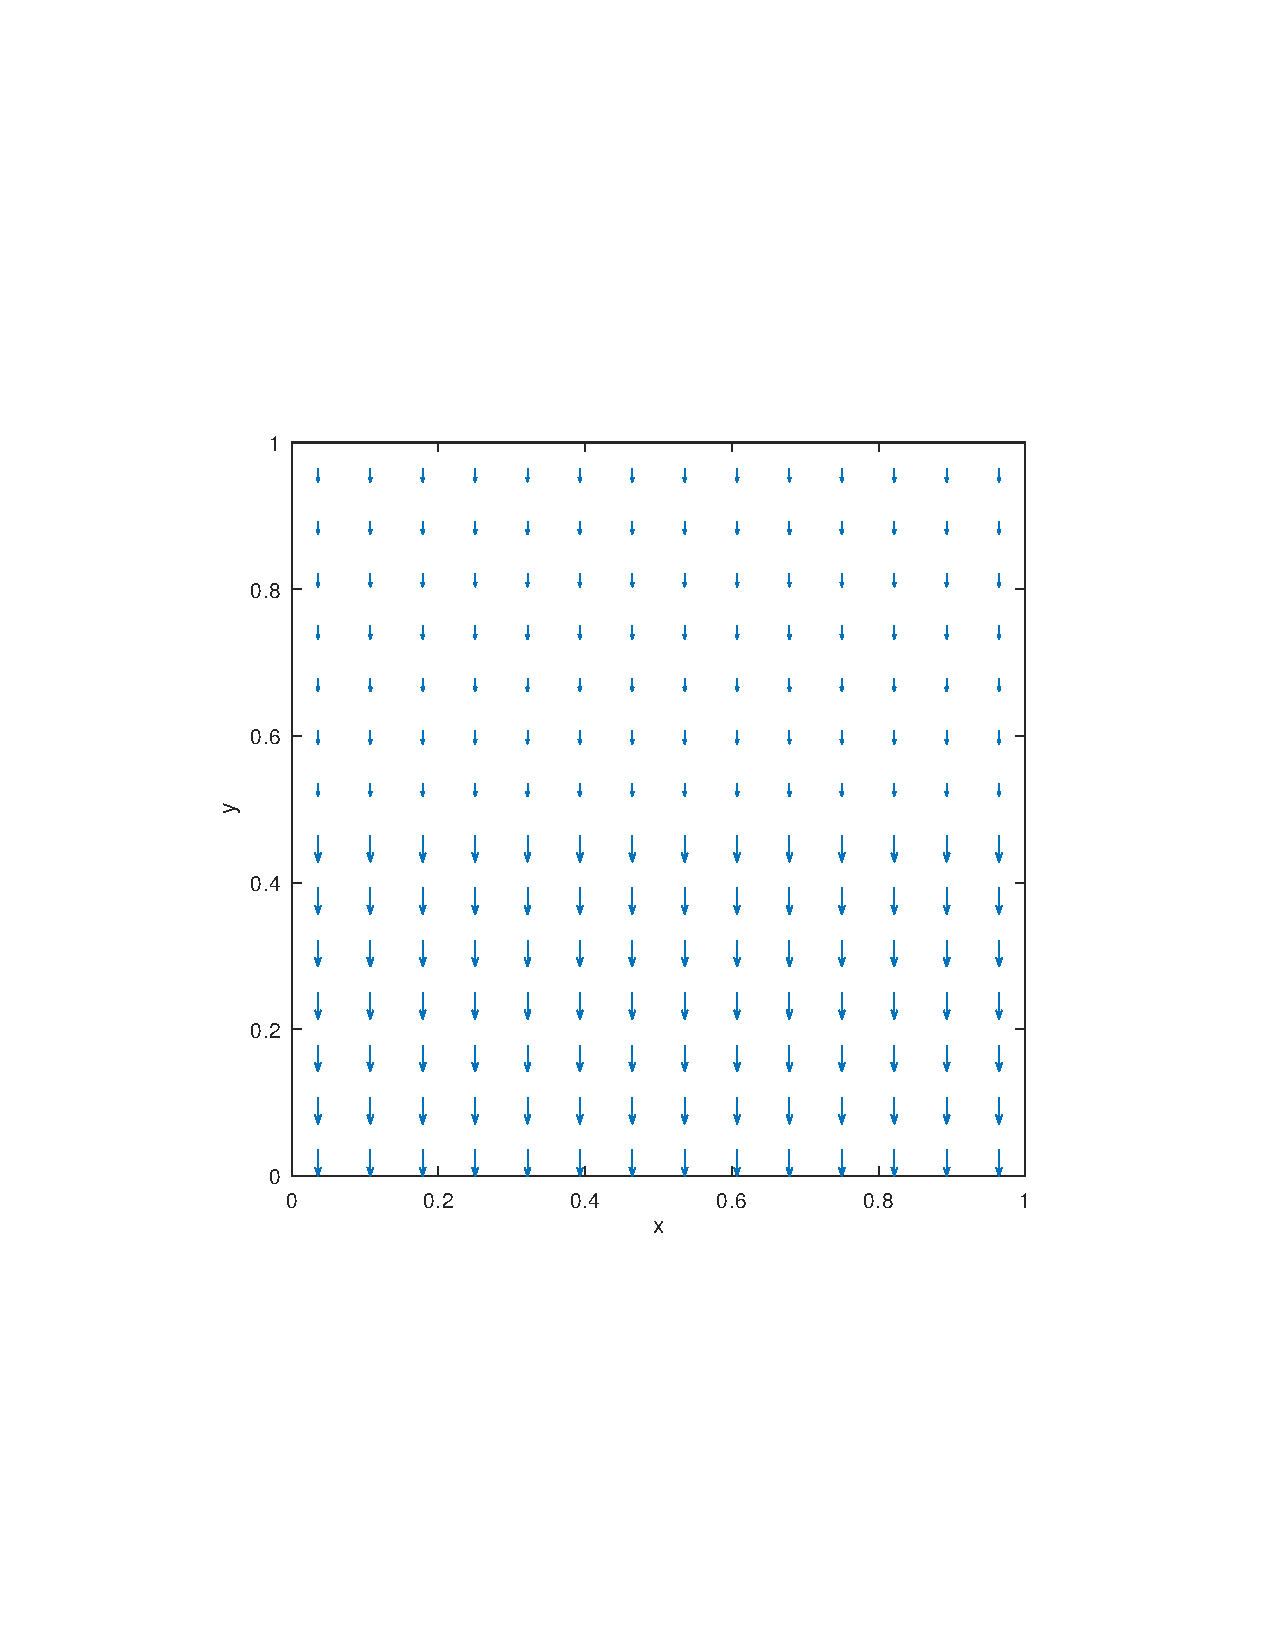
\includegraphics[trim = 20mm 70mm 20mm 70mm, clip,width=0.7\linewidth]{E_2D_B.pdf}
	\caption{Numerisch bestimmter Verlauf des elektrischen Feldes des Kondensators aus \ref{exer:calcCapsAnalytical}.1 5b$)$ in 2D}
\end{figure}

\begin{figure}[h!]
	\centering
	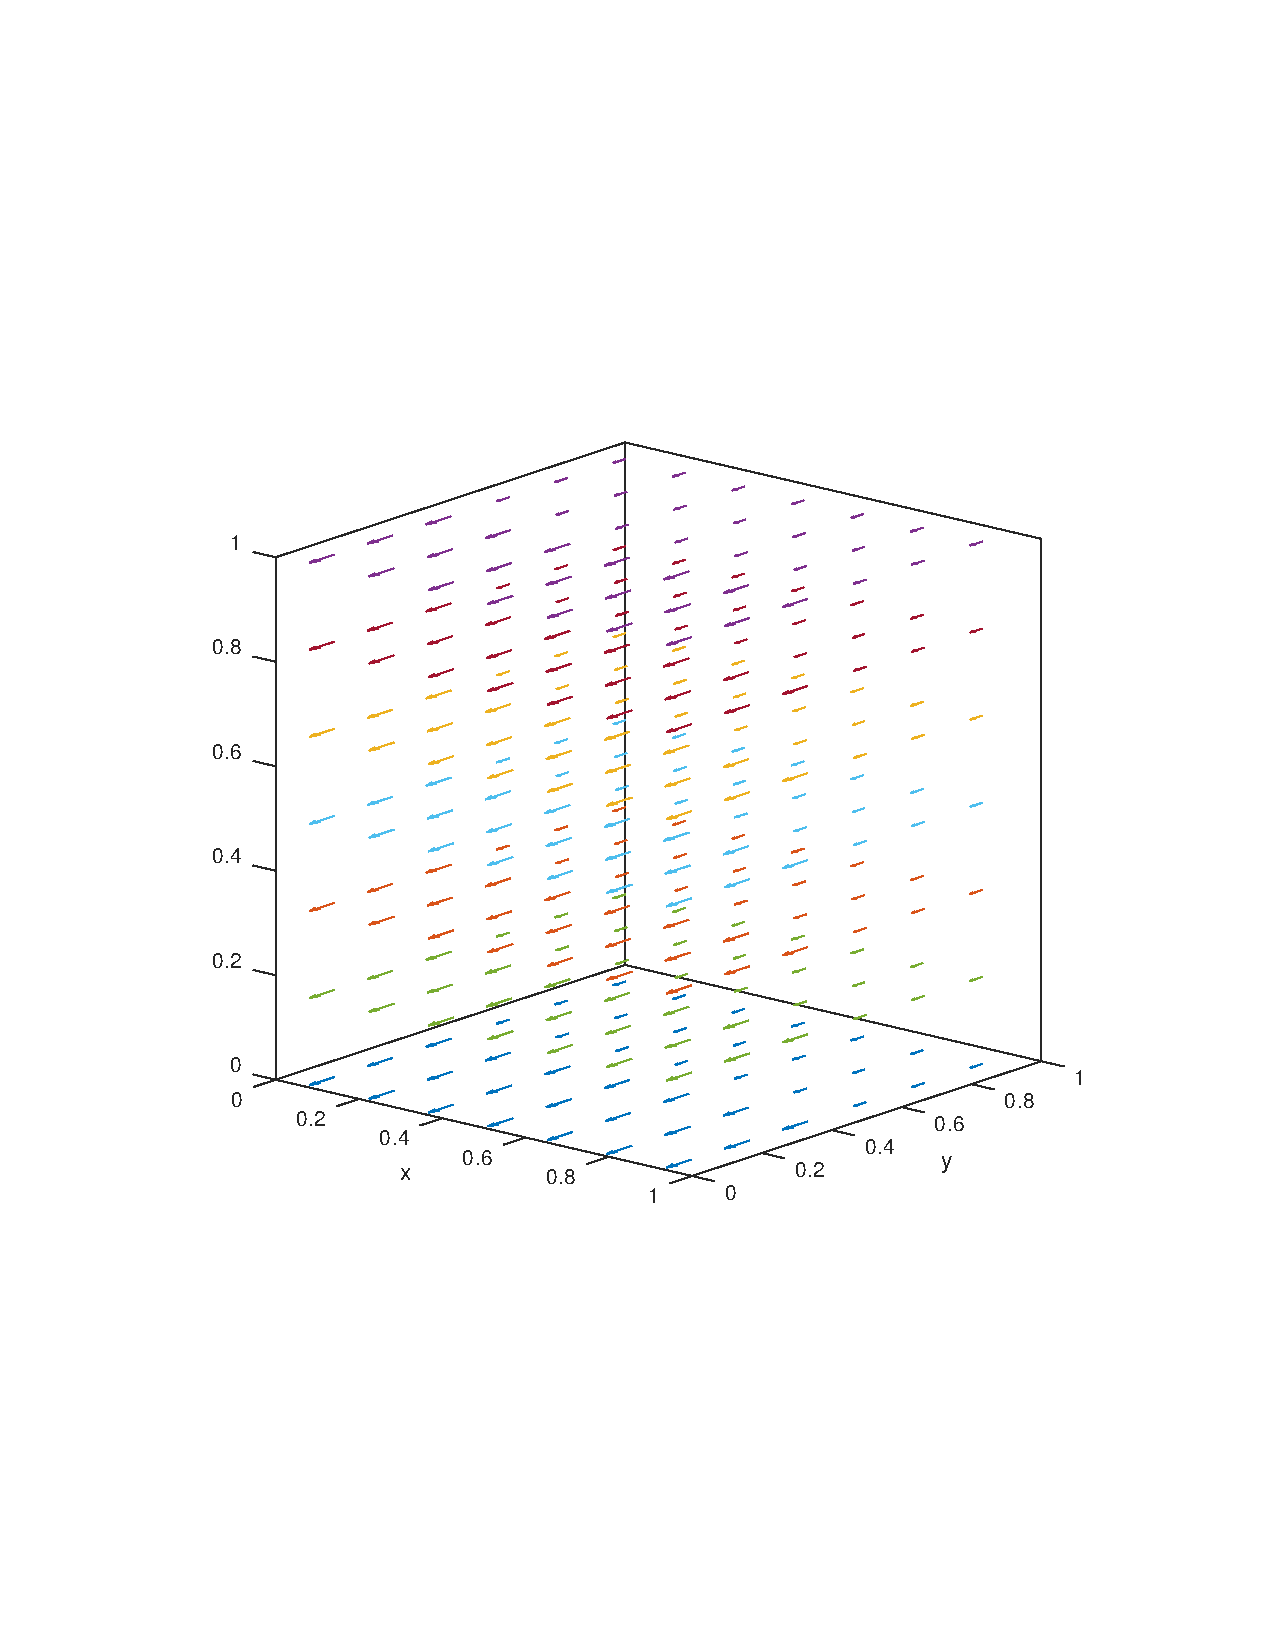
\includegraphics[trim = 20mm 70mm 20mm 70mm, clip,width=0.7\linewidth]{E_3D_B.pdf}
	\caption{Numerisch bestimmter Verlauf des elektrischen Feldes des Kondensators aus \ref{exer:calcCapsAnalytical}.1 5b$)$ in 3D}
\end{figure}

\begin{figure}[h!]
	\centering
	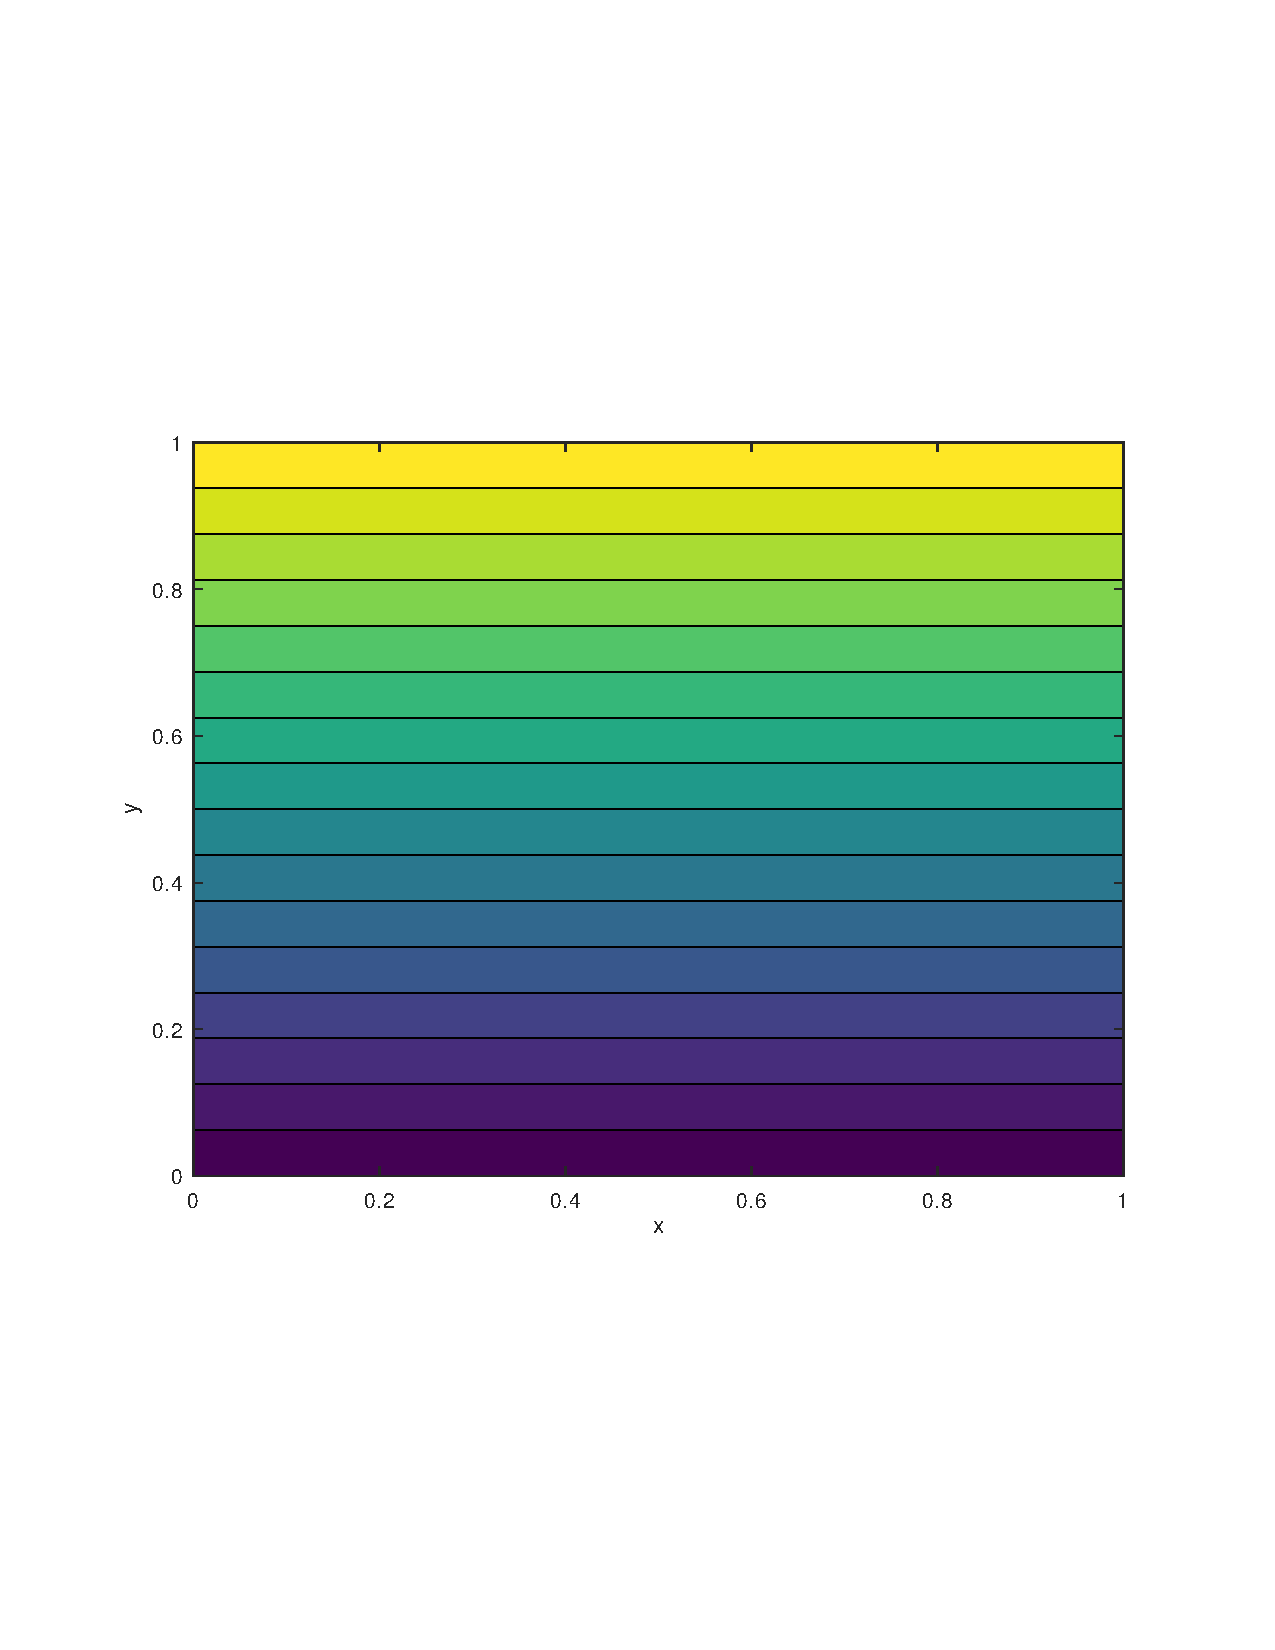
\includegraphics[trim = 20mm 70mm 20mm 70mm, clip,width=0.7\linewidth]{potential_C.pdf}
	\caption{Numerisch bestimmter Potentialverlauf des Kondensators aus \ref{exer:calcCapsAnalytical}.1 5c$)$}
\end{figure}

\begin{figure}[h!]
	\centering
	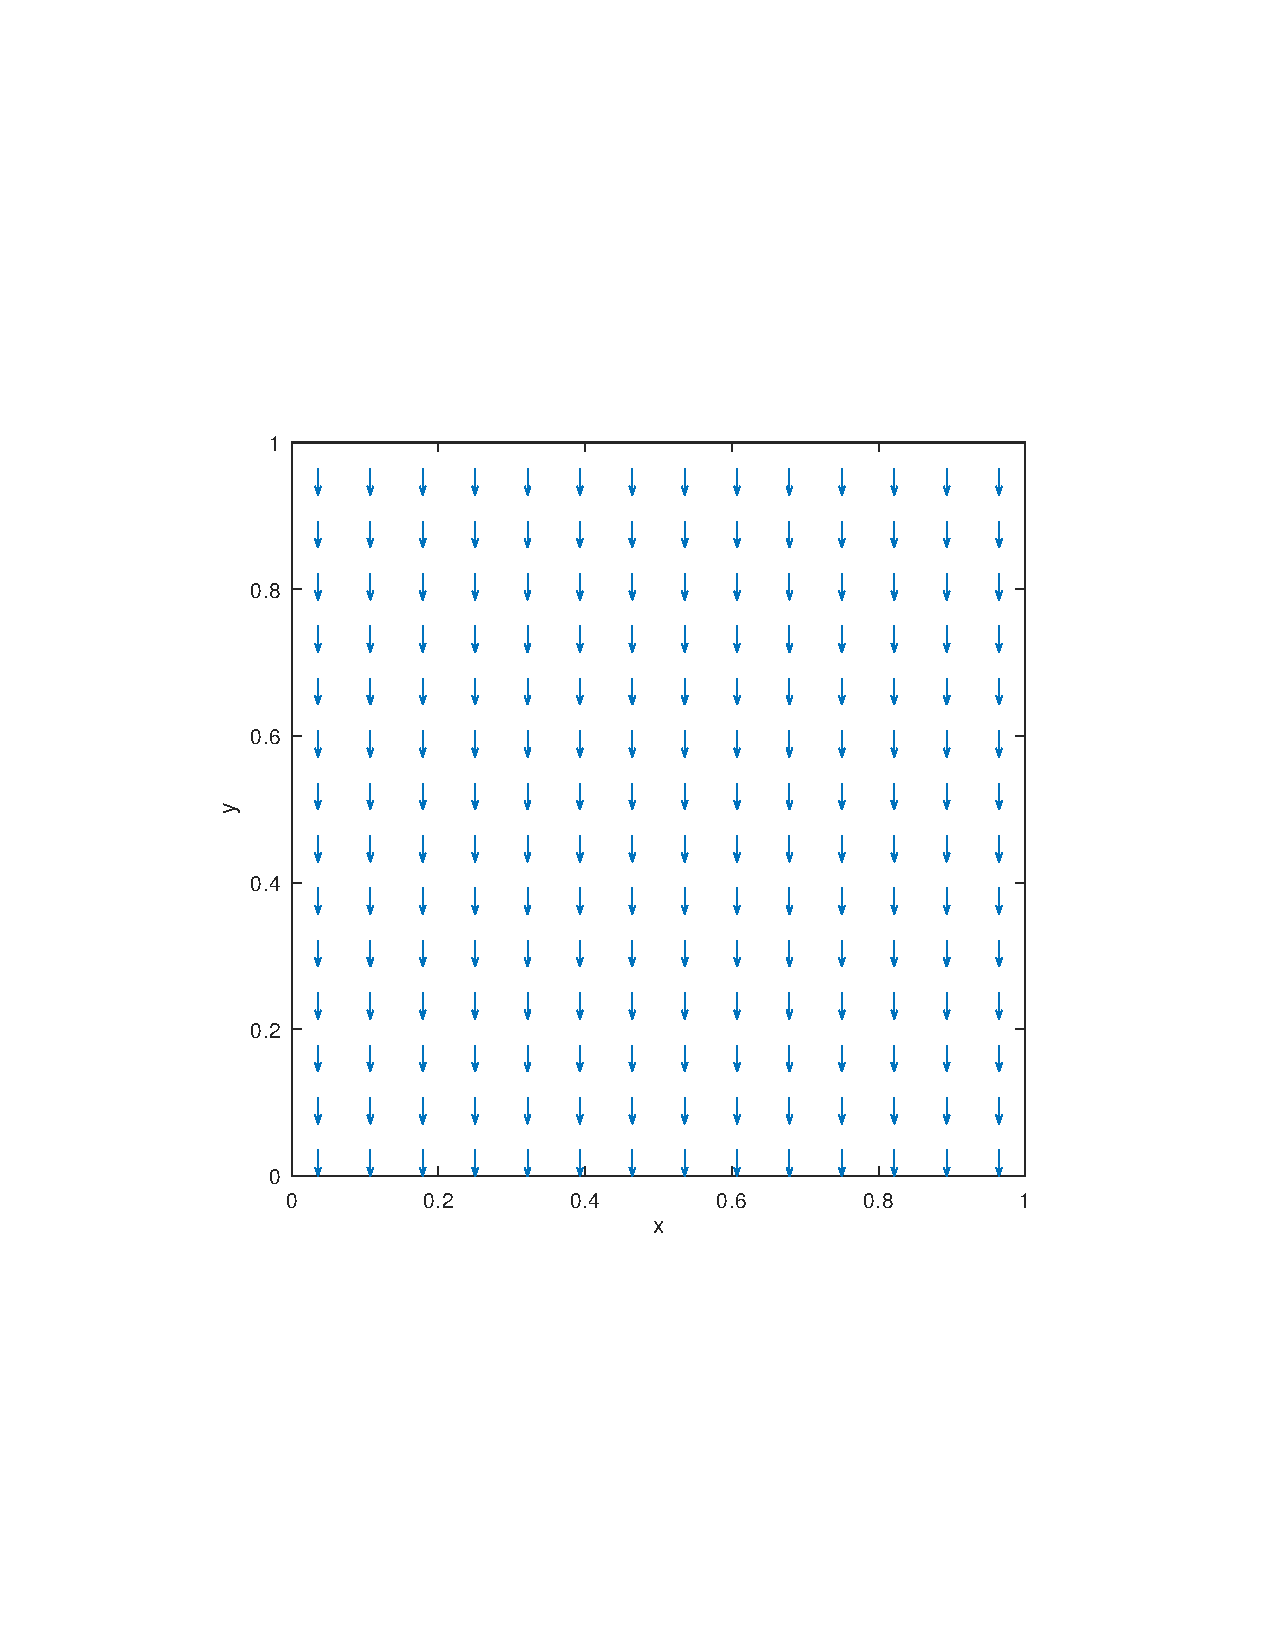
\includegraphics[trim = 20mm 70mm 20mm 70mm, clip,width=0.7\linewidth]{E_2D_C.pdf}
	\caption{Numerisch bestimmter Verlauf des elektrischen Feldes des Kondensators aus \ref{exer:calcCapsAnalytical}.1 5c$)$ in 2D}
\end{figure}

\begin{figure}[h!]
	\centering
	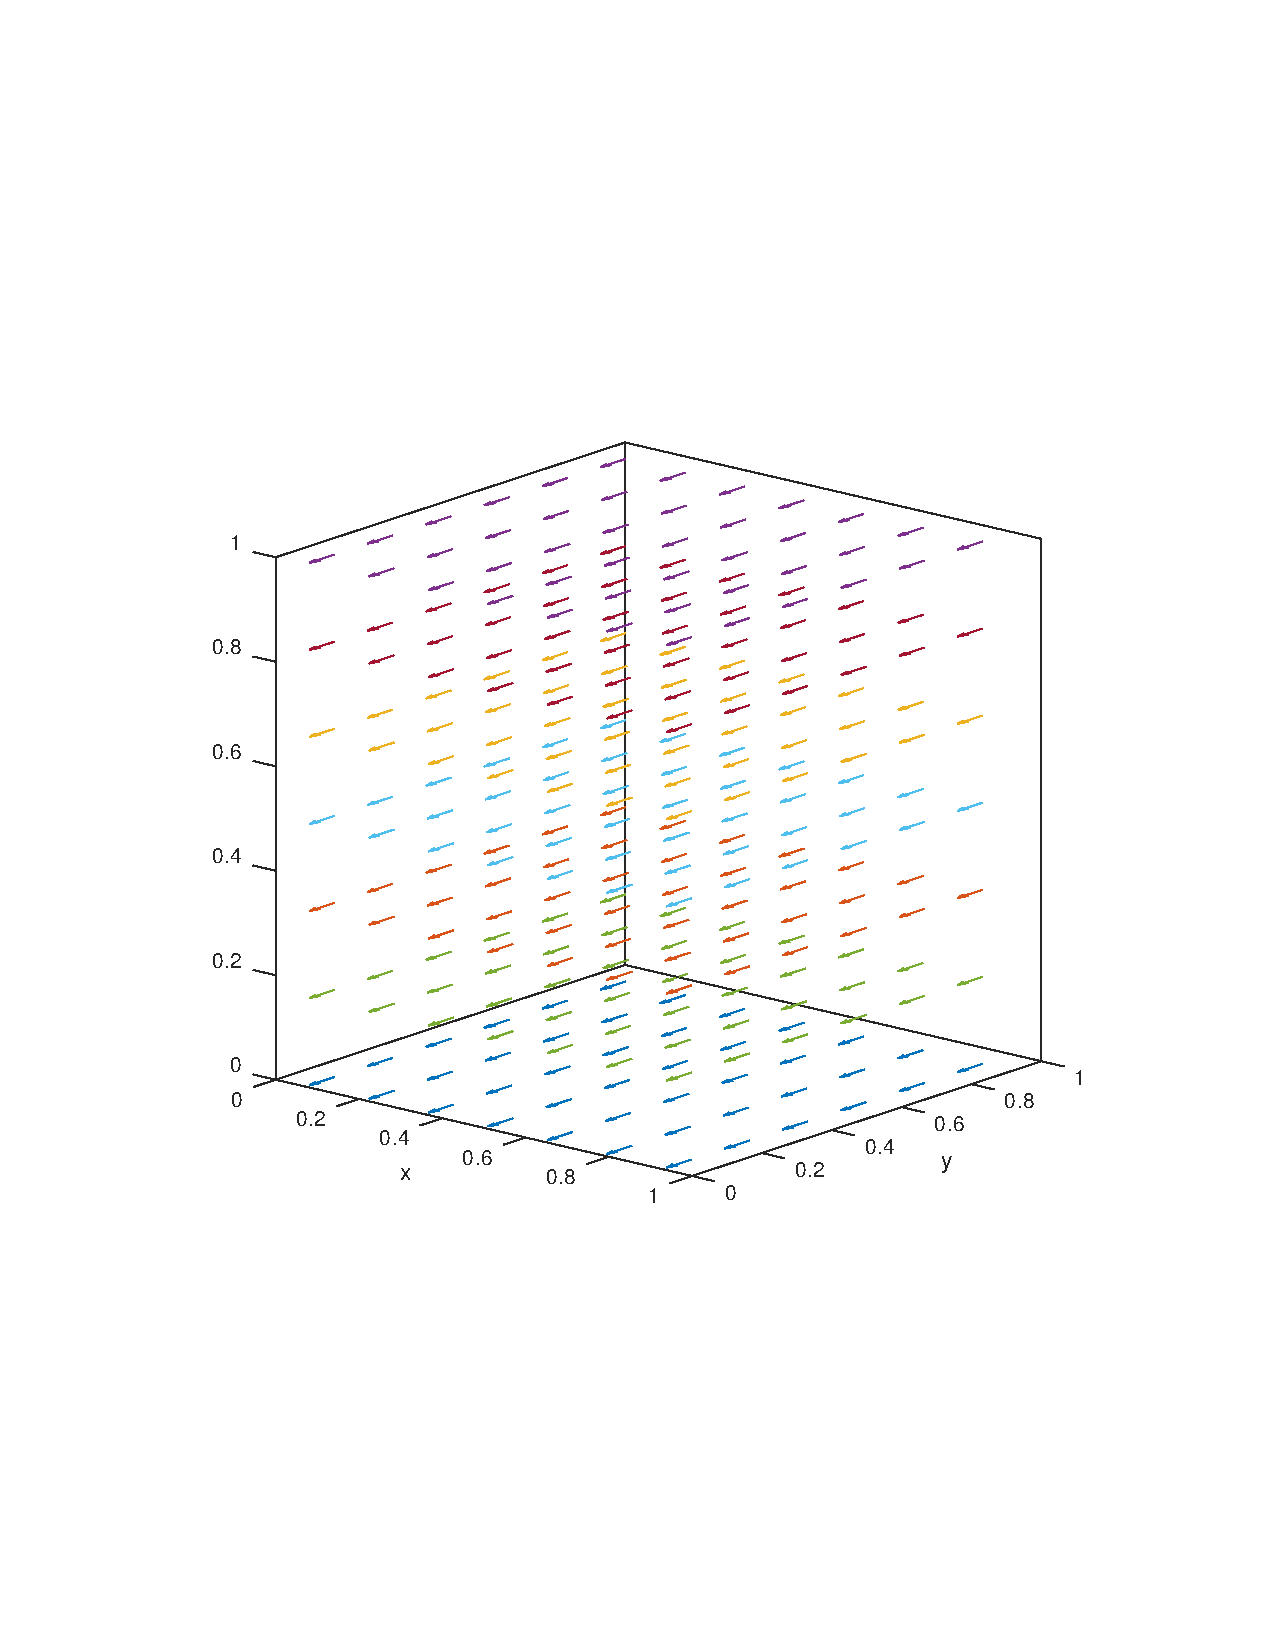
\includegraphics[trim = 20mm 70mm 20mm 70mm, clip,width=0.7\linewidth]{E_3D_C.pdf}
	\caption{Numerisch bestimmter Verlauf des elektrischen Feldes des Kondensators aus \ref{exer:calcCapsAnalytical}.1 5c$)$ in 3D}
\end{figure}

\begin{figure}[h!]
	\centering
	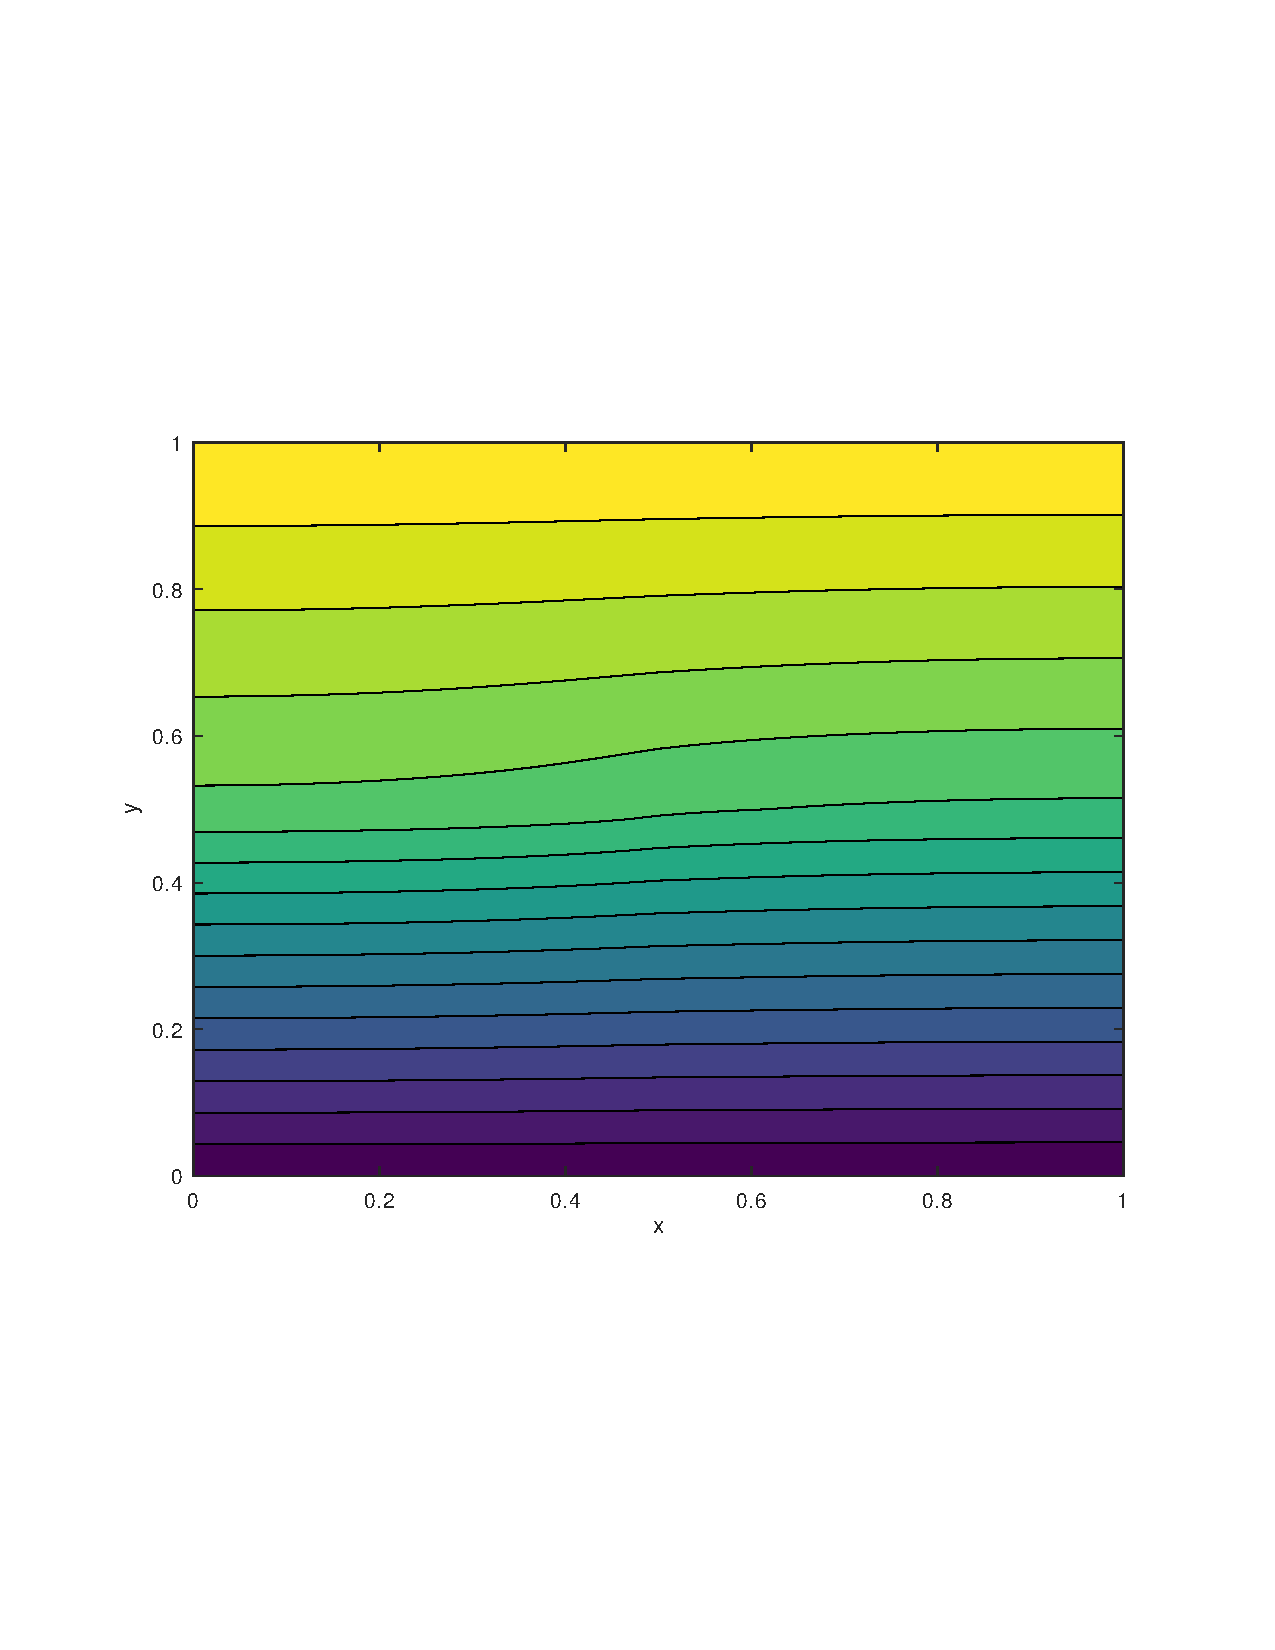
\includegraphics[trim = 20mm 70mm 20mm 70mm, clip,width=0.7\linewidth]{potential_D.pdf}
	\caption{Numerisch bestimmter Potentialverlauf des Kondensators aus \ref{exer:calcCapsAnalytical}.1 5d$)$}
\end{figure}

\begin{figure}[h!]
	\centering
	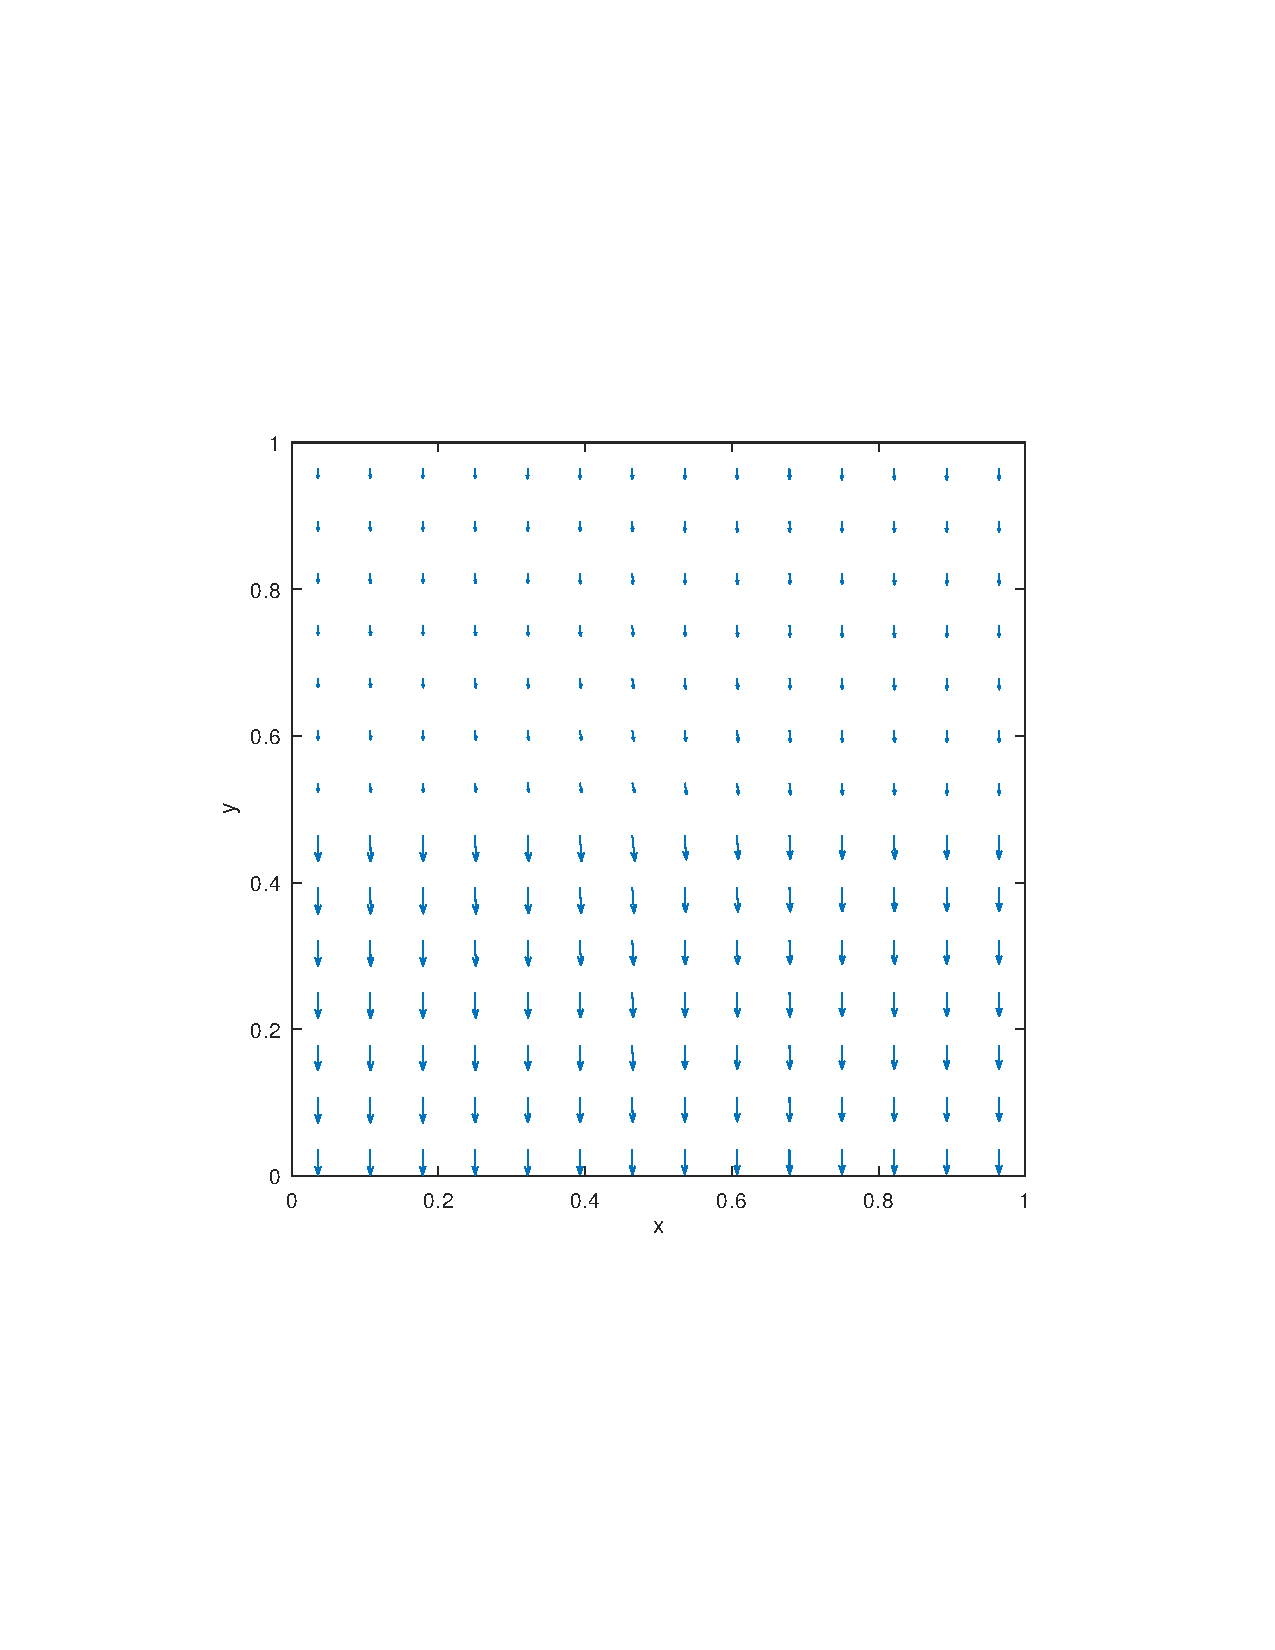
\includegraphics[trim = 20mm 70mm 20mm 70mm, clip,width=0.7\linewidth]{E_2D_D.pdf}
	\caption{Numerisch bestimmter Verlauf des elektrischen Feldes des Kondensators aus \ref{exer:calcCapsAnalytical}.1 5d$)$ in 2D}
\end{figure}

\begin{figure}[h!]
	\centering
	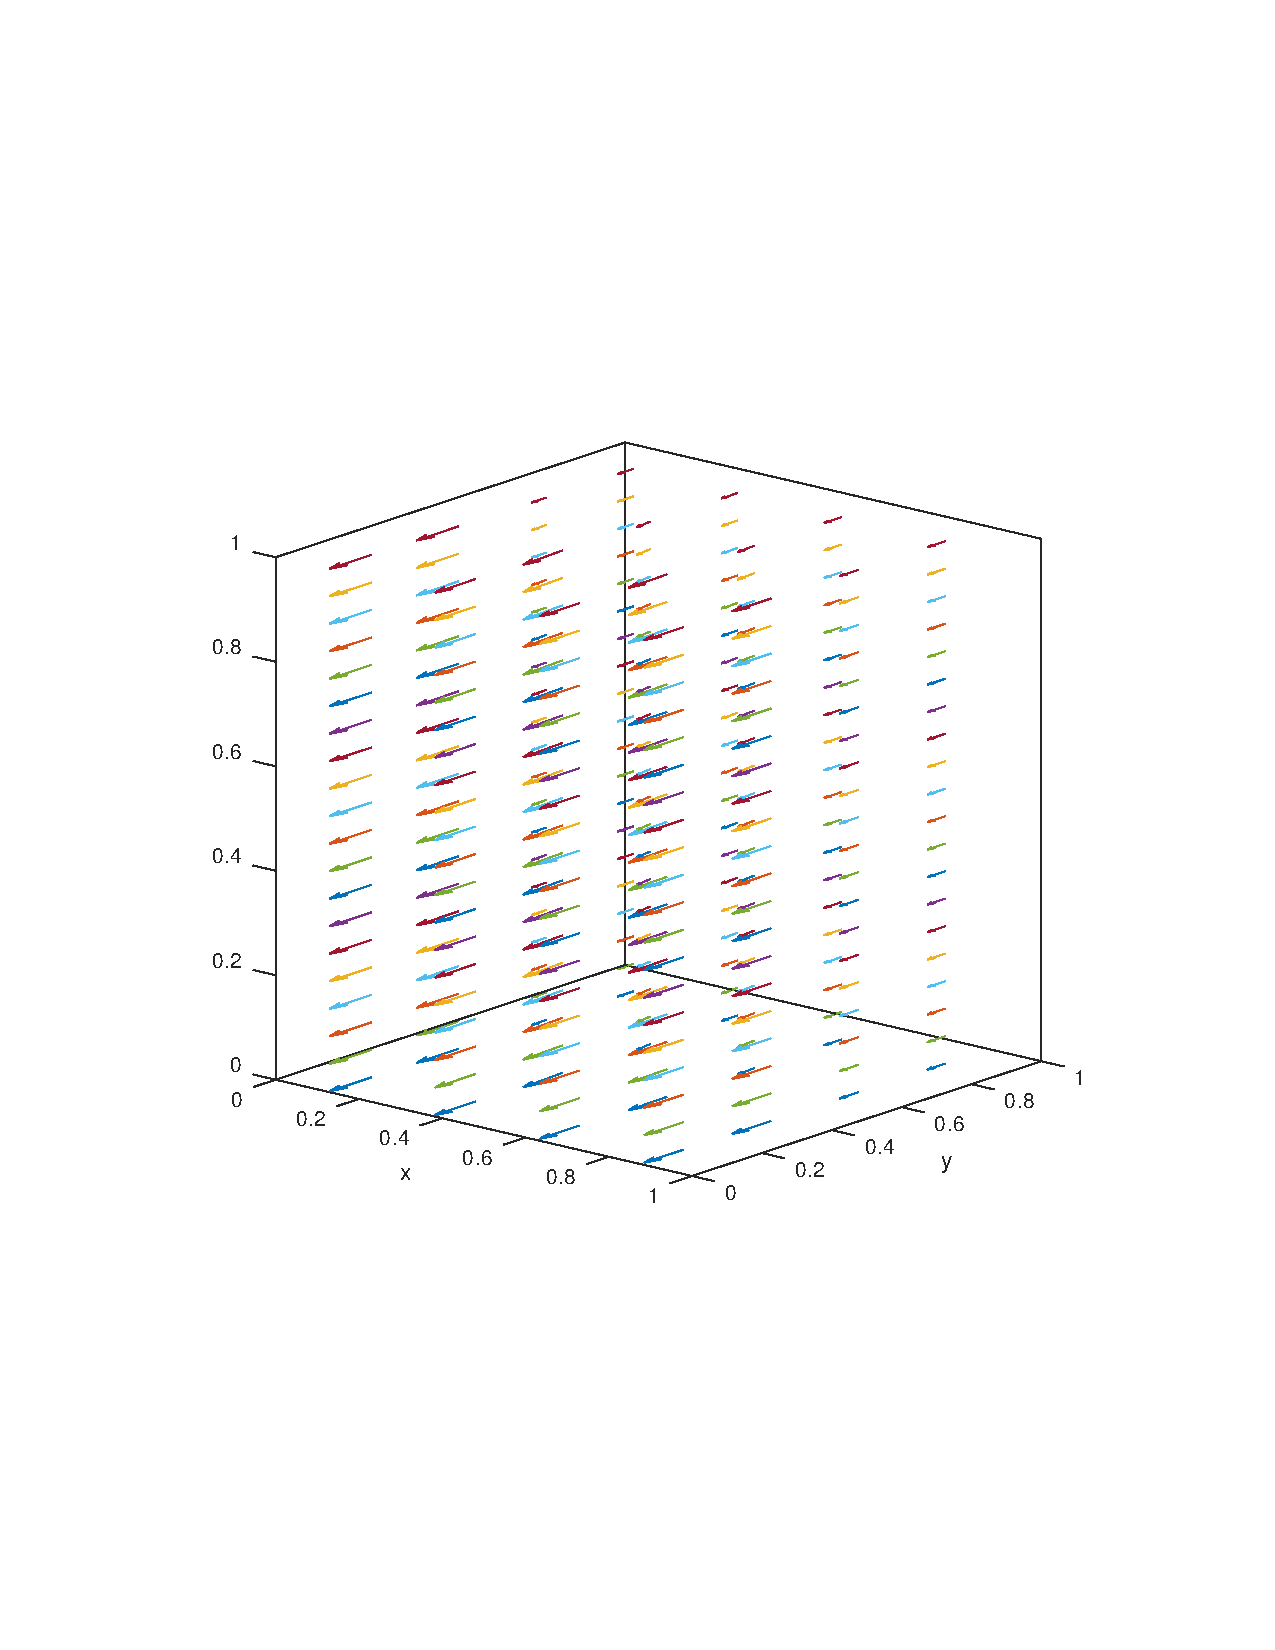
\includegraphics[trim = 20mm 70mm 20mm 70mm, clip,width=0.7\linewidth]{E_3D_D.pdf}
	\caption{Numerisch bestimmter Verlauf des elektrischen Feldes des Kondensators aus \ref{exer:calcCapsAnalytical}.1 5d$)$ in 3D}
\end{figure}

\begin{figure}[h!]
	\centering
	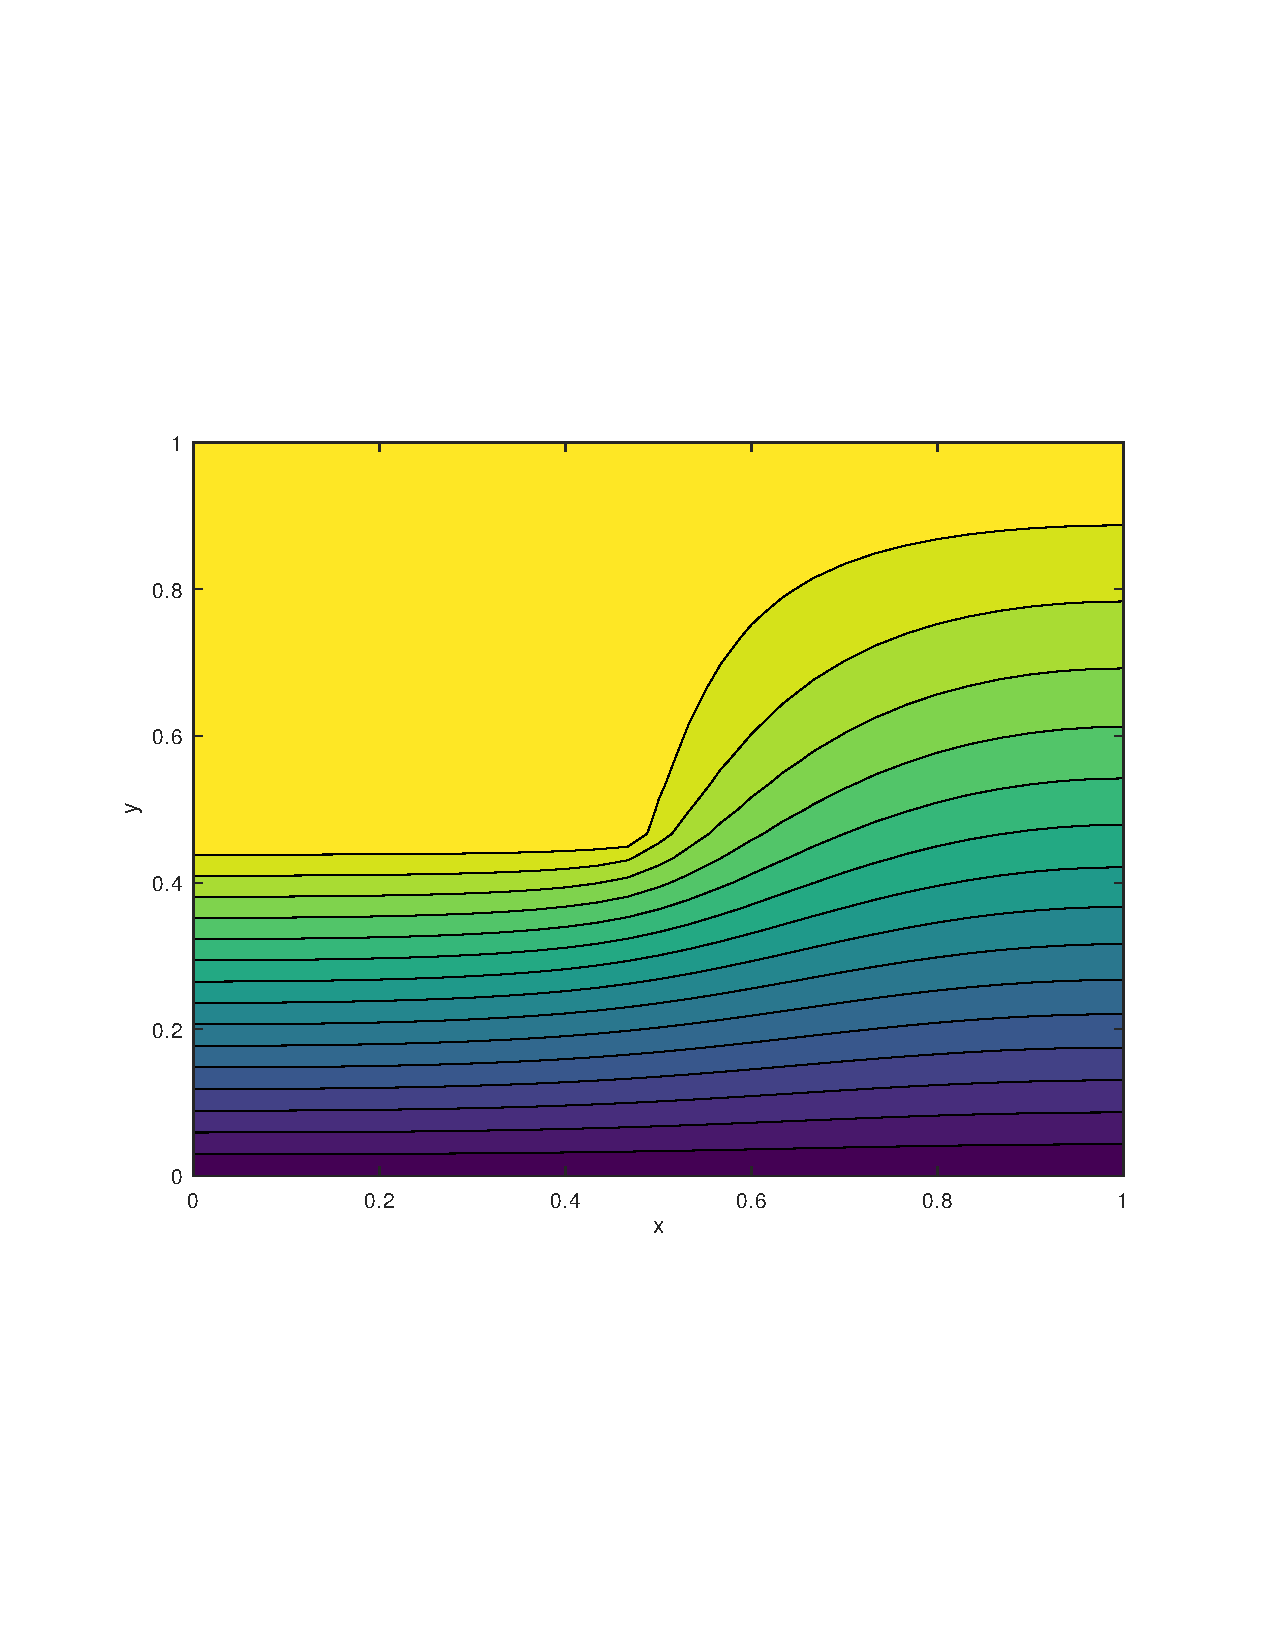
\includegraphics[trim = 20mm 70mm 20mm 70mm, clip,width=0.7\linewidth]{potential_E.pdf}
	\caption{Numerisch bestimmter Potentialverlauf des Kondensators aus \ref{exer:calcCapsAnalytical}.1 5e$)$}
\end{figure}

\begin{figure}[h!]
	\centering
	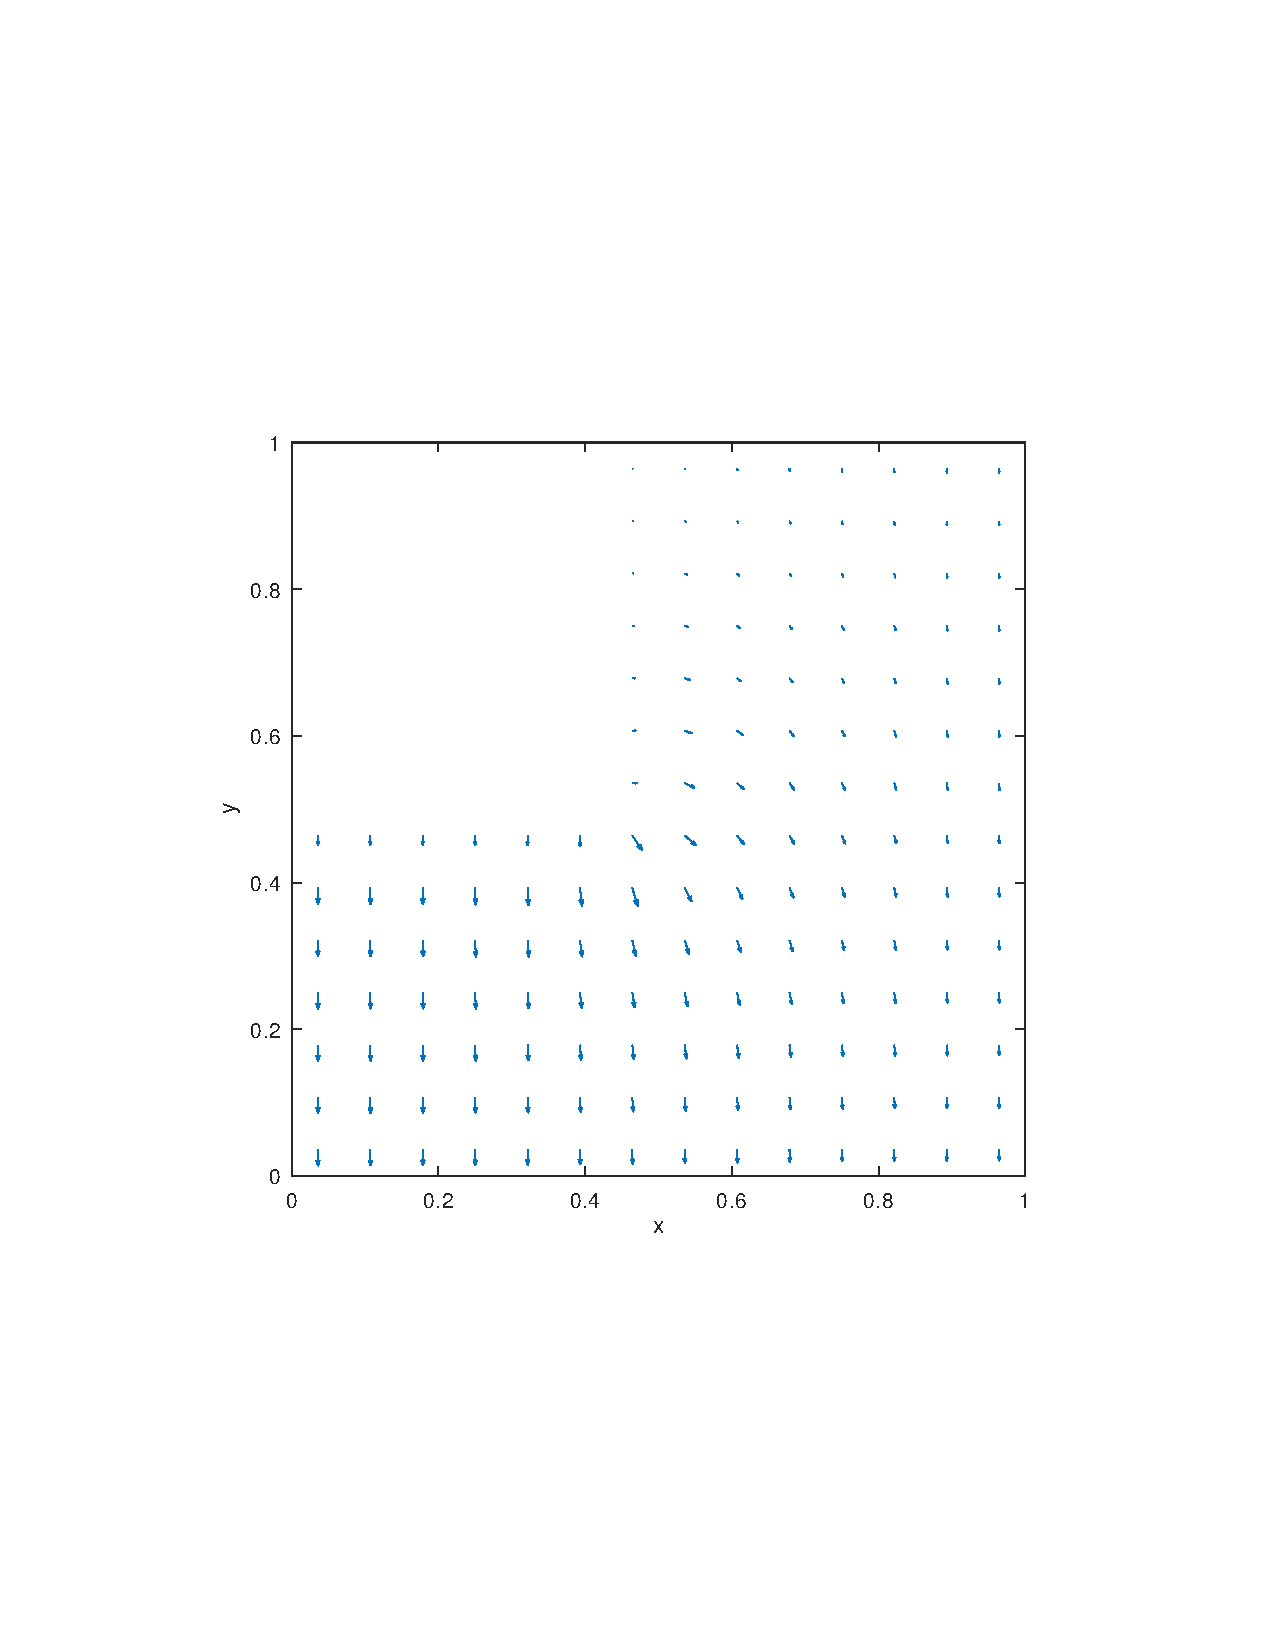
\includegraphics[trim = 20mm 70mm 20mm 70mm, clip,width=0.7\linewidth]{E_2D_E.pdf}
	\caption{Numerisch bestimmter Verlauf des elektrischen Feldes des Kondensators aus \ref{exer:calcCapsAnalytical}.1 5e$)$ in 2D}
\end{figure}

\begin{figure}[h!]
	\centering
	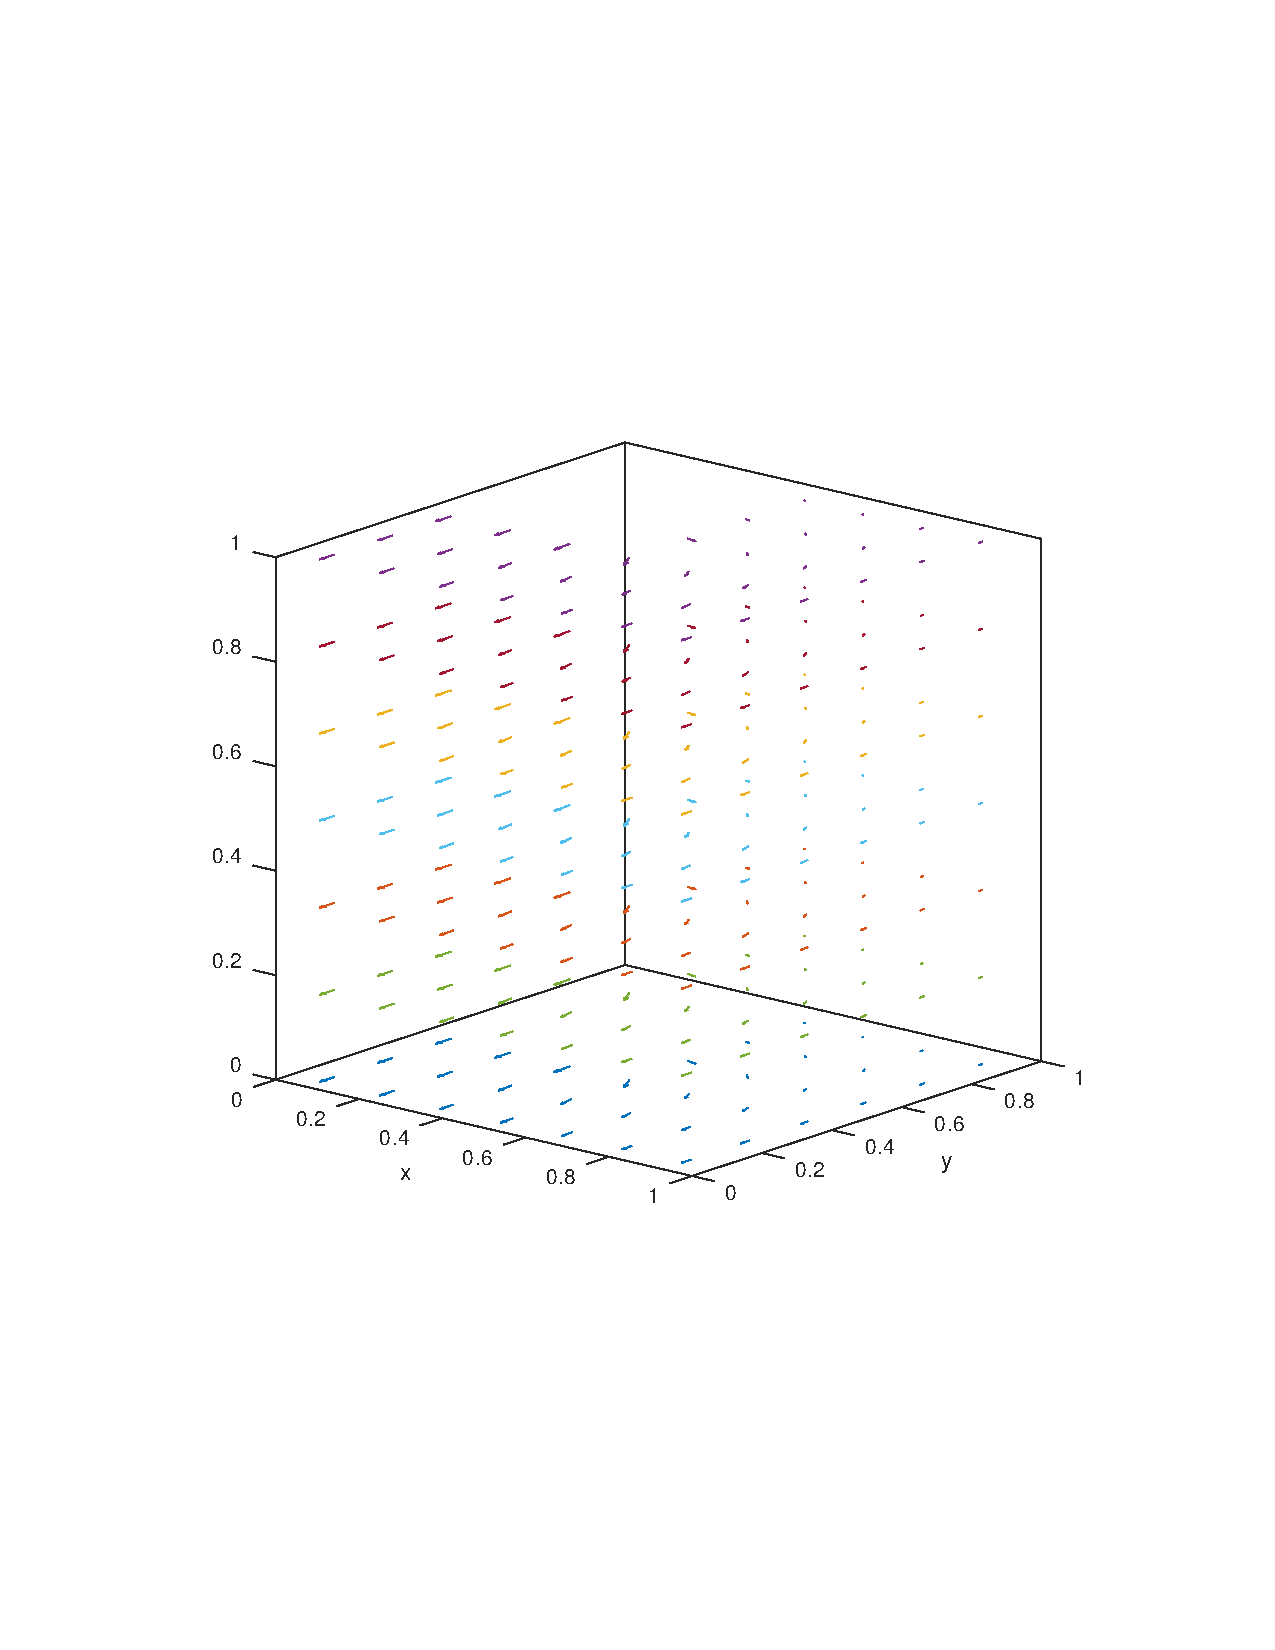
\includegraphics[trim = 20mm 70mm 20mm 70mm, clip,width=0.7\linewidth]{E_3D_E.pdf}
	\caption{Numerisch bestimmter Verlauf des elektrischen Feldes des Kondensators aus \ref{exer:calcCapsAnalytical}.1 5e$)$ in 3D}
	\label{fig:C_5e_3D}
\end{figure}

\begin{figure}[ht]
	\centering
	\def\svgwidth{0.7\textwidth}
	\input{diffstern.pdf_tex}
	\caption{Differenzenstern}
	\label{fig:diffstern}
\end{figure}

\begin{figure}
	\centering
	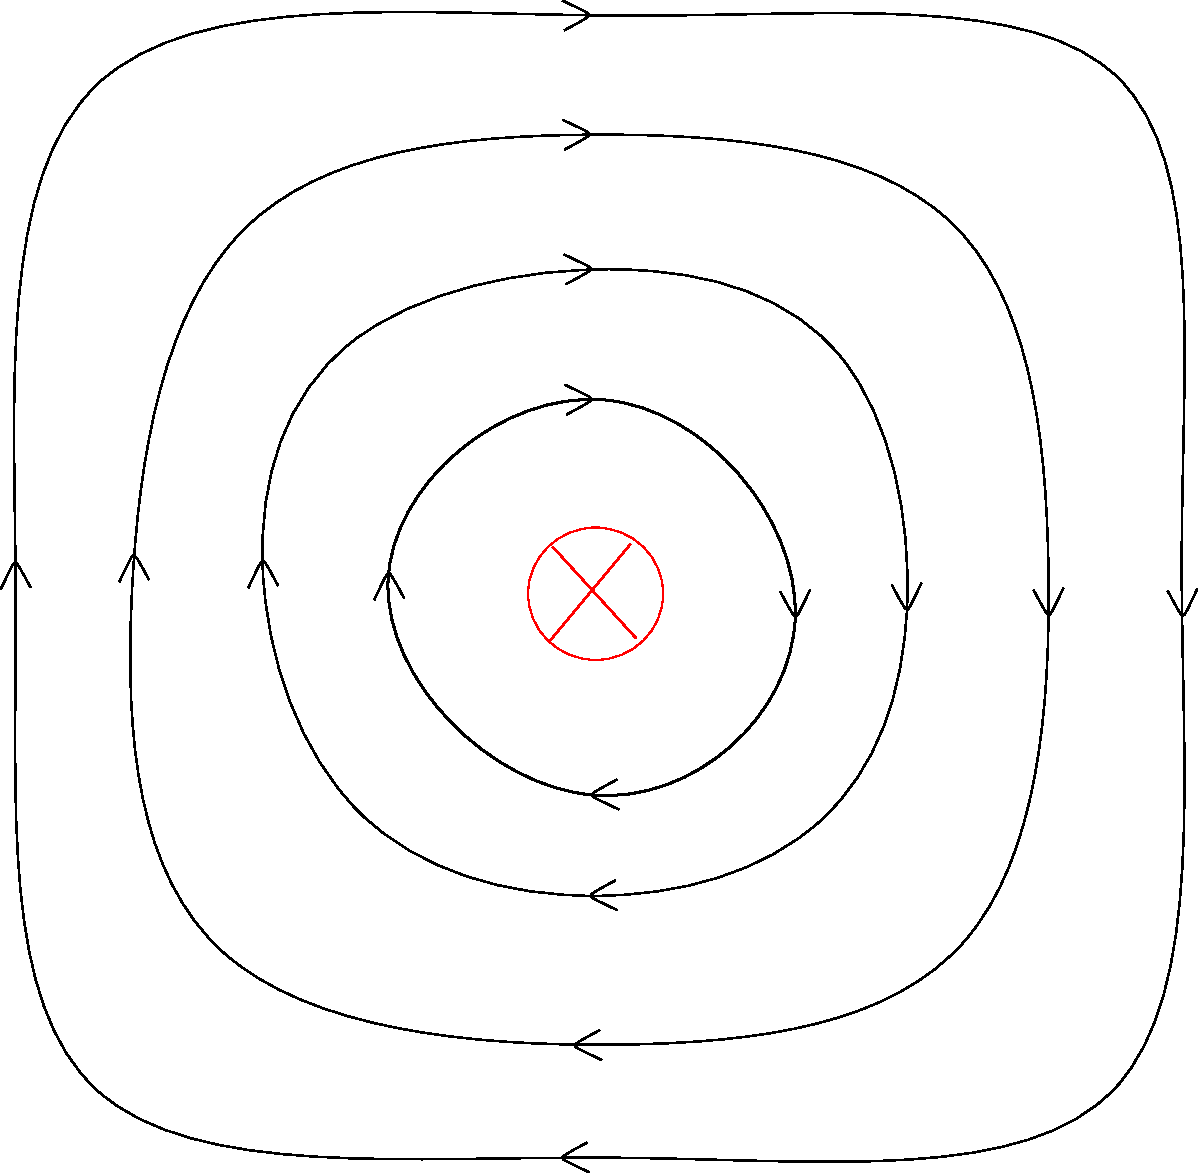
\includegraphics[width=0.5\linewidth]{NeumannRand}
	\caption{Skizze des Magnetfeldes eines Linienleiters mit Neumannrandbedingungen}
	\label{fig:neumannrand}
\end{figure}

\begin{figure}
	\centering
	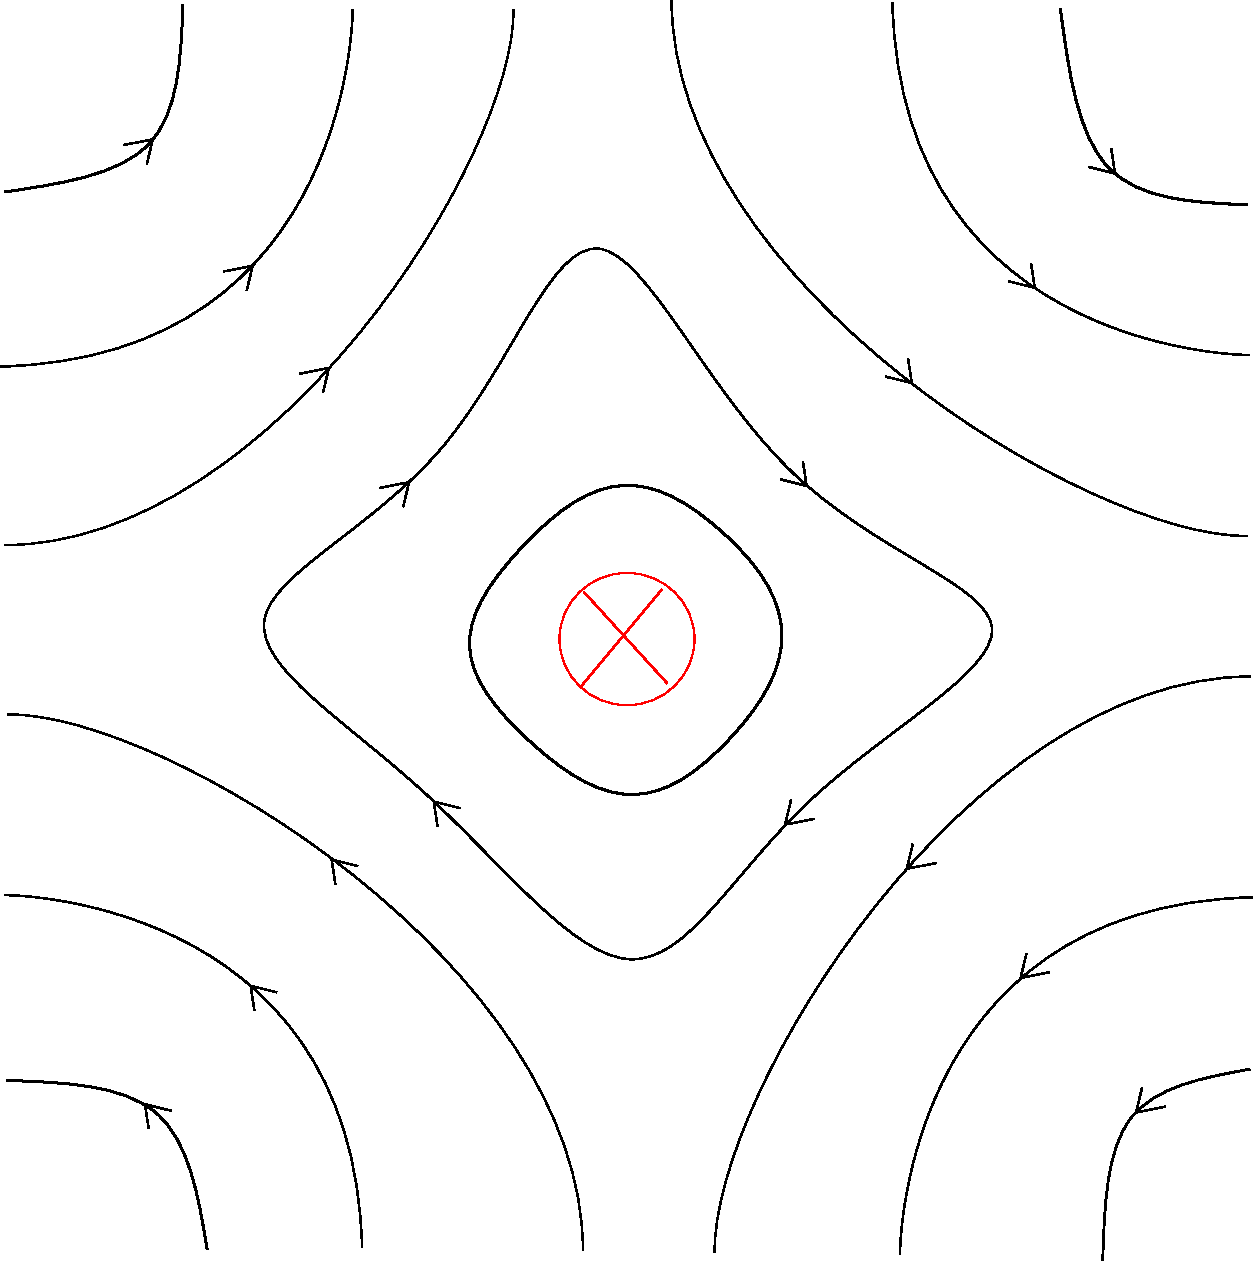
\includegraphics[width=0.5\linewidth]{DirichletRand}
	\caption{Skizze des Magnetfeldes eines Linienleiters mit Dirichletrandbedingungen}
	\label{fig:dirichletrand}
\end{figure}
\begin{figure}[ht]
	\centering
	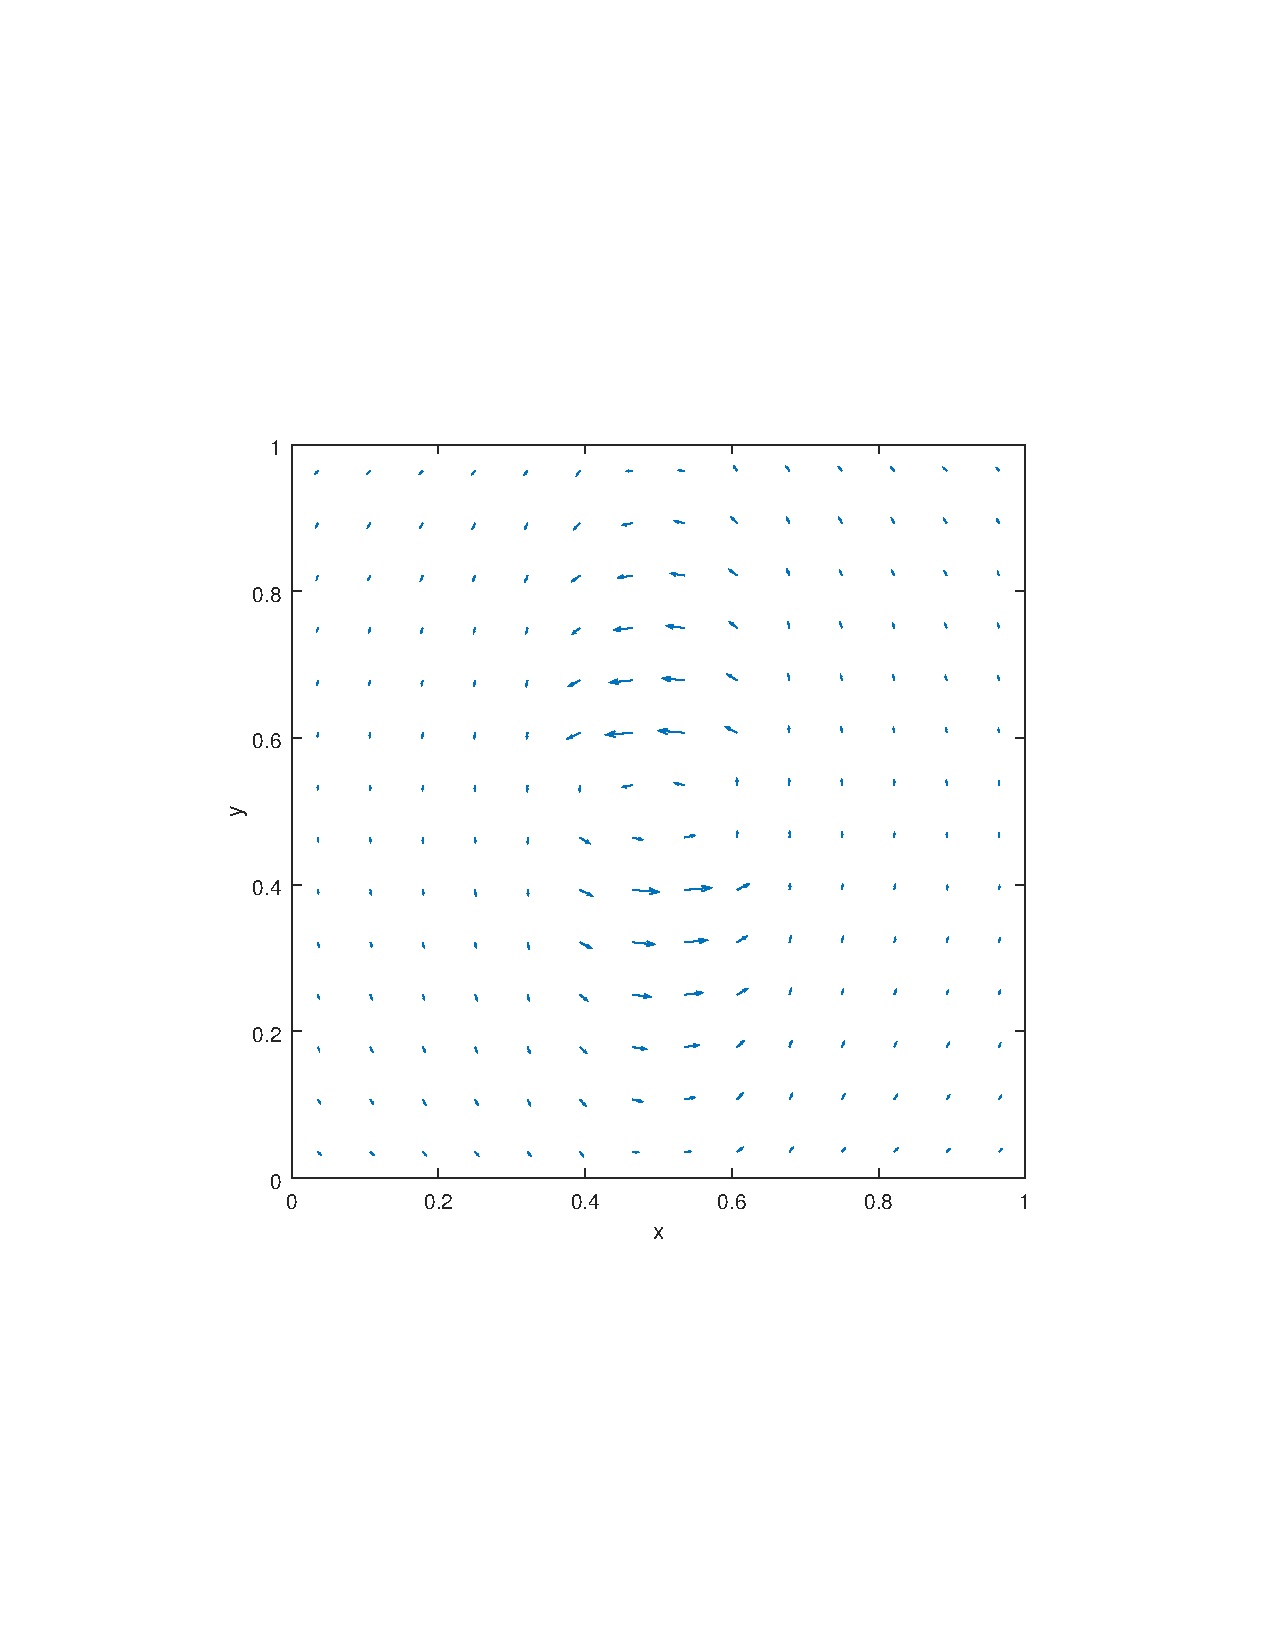
\includegraphics[width=0.8\linewidth]{Plot_der_hilffelders.pdf}
	\caption{Graphische Darstellung des Hilffeldes $\hfit_{\text{i}}$ }
	\label{fig:hilffeld}
\end{figure}

\begin{figure}[hb]
	\centering
	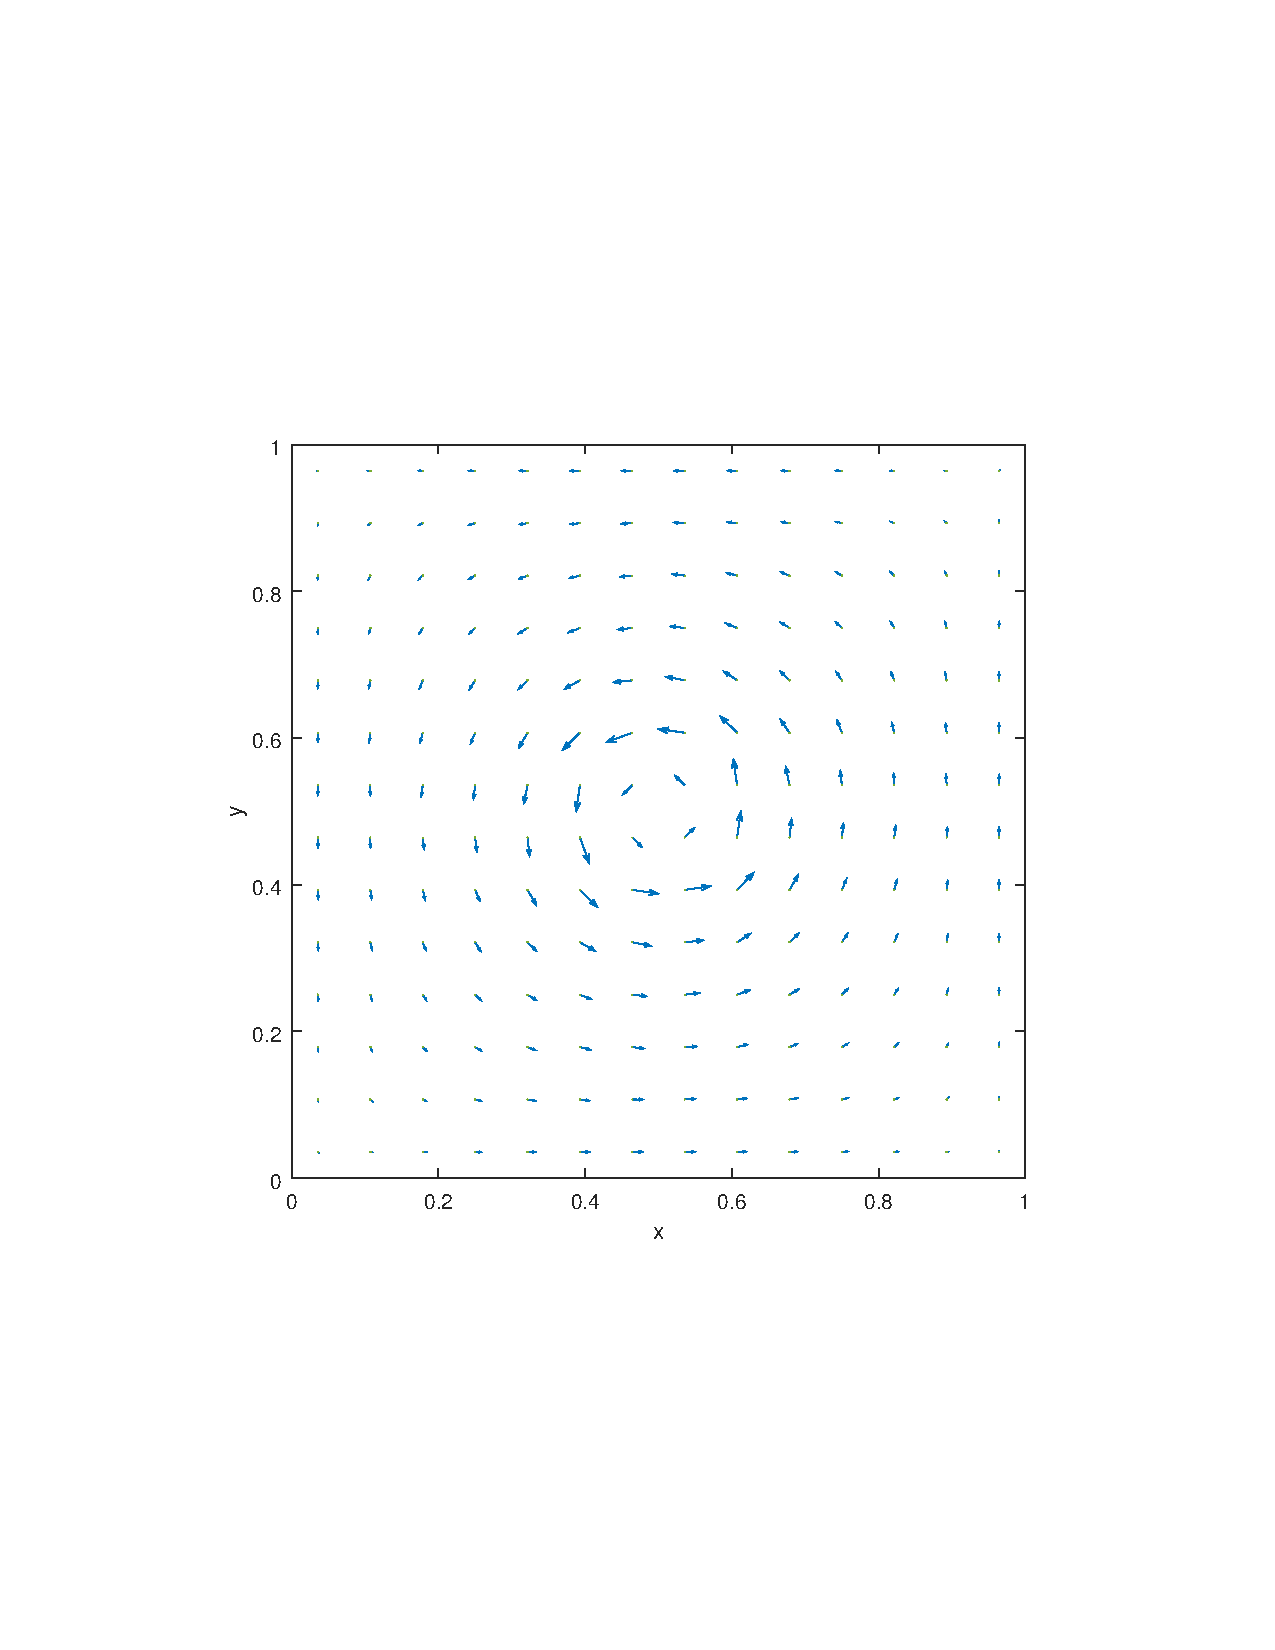
\includegraphics[width=0.8\linewidth]{homoFeld.pdf}
	\caption{homogenes $\vec{H}$-Feld  }
	\label{fig:homfeld}
\end{figure}

\begin{figure}[hb]
	\centering
	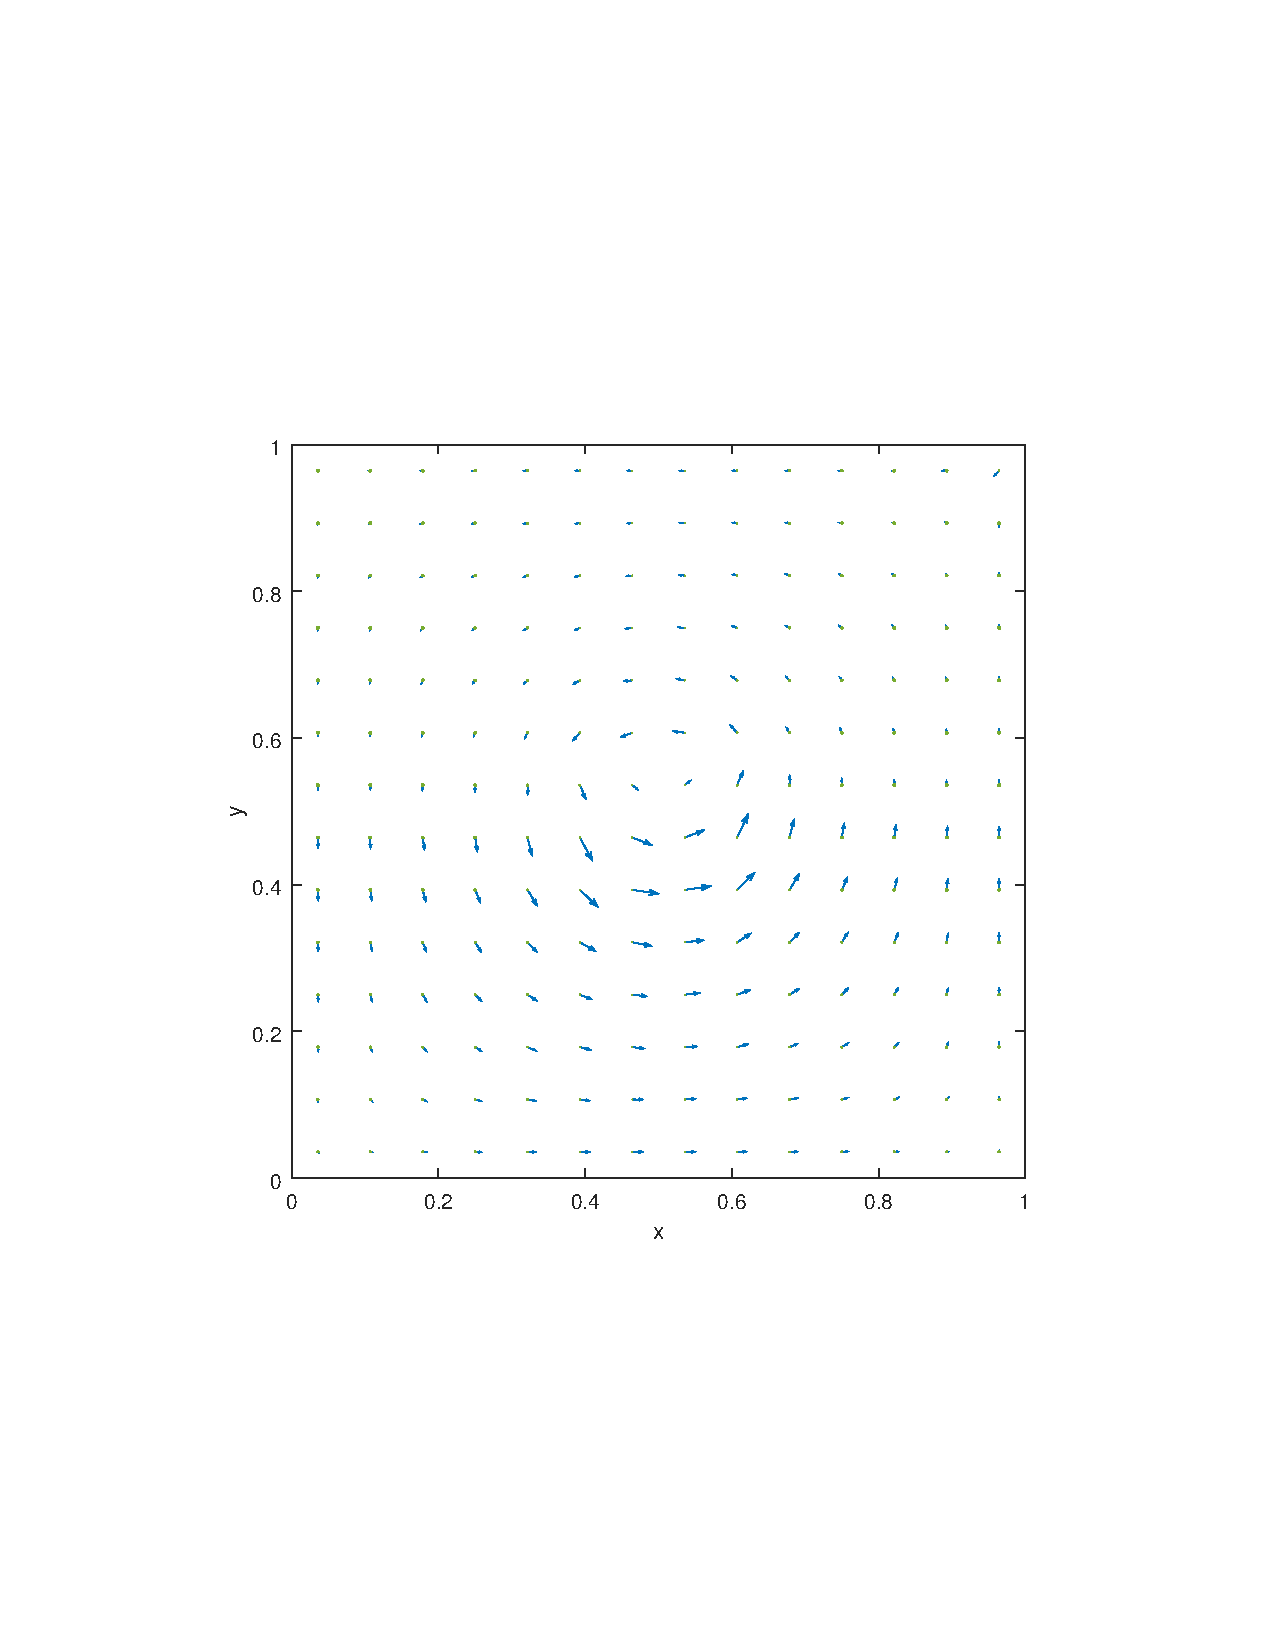
\includegraphics[width=0.8\linewidth]{inhomoFeld.pdf}
	\caption{inhomogenes $\vec{H}$-Feld mit $\mu_1=1$ und $\mu_2=5$   }
	\label{fig:inhomfeld}
\end{figure}

\end{document}
